\subsection{Sơ đồ tuần tự}
% --- NHÓM 1: XÁC THỰC NGƯỜI DÙNG (AUTHENTICATION) ---

\begin{figure}[H]
    \centering
    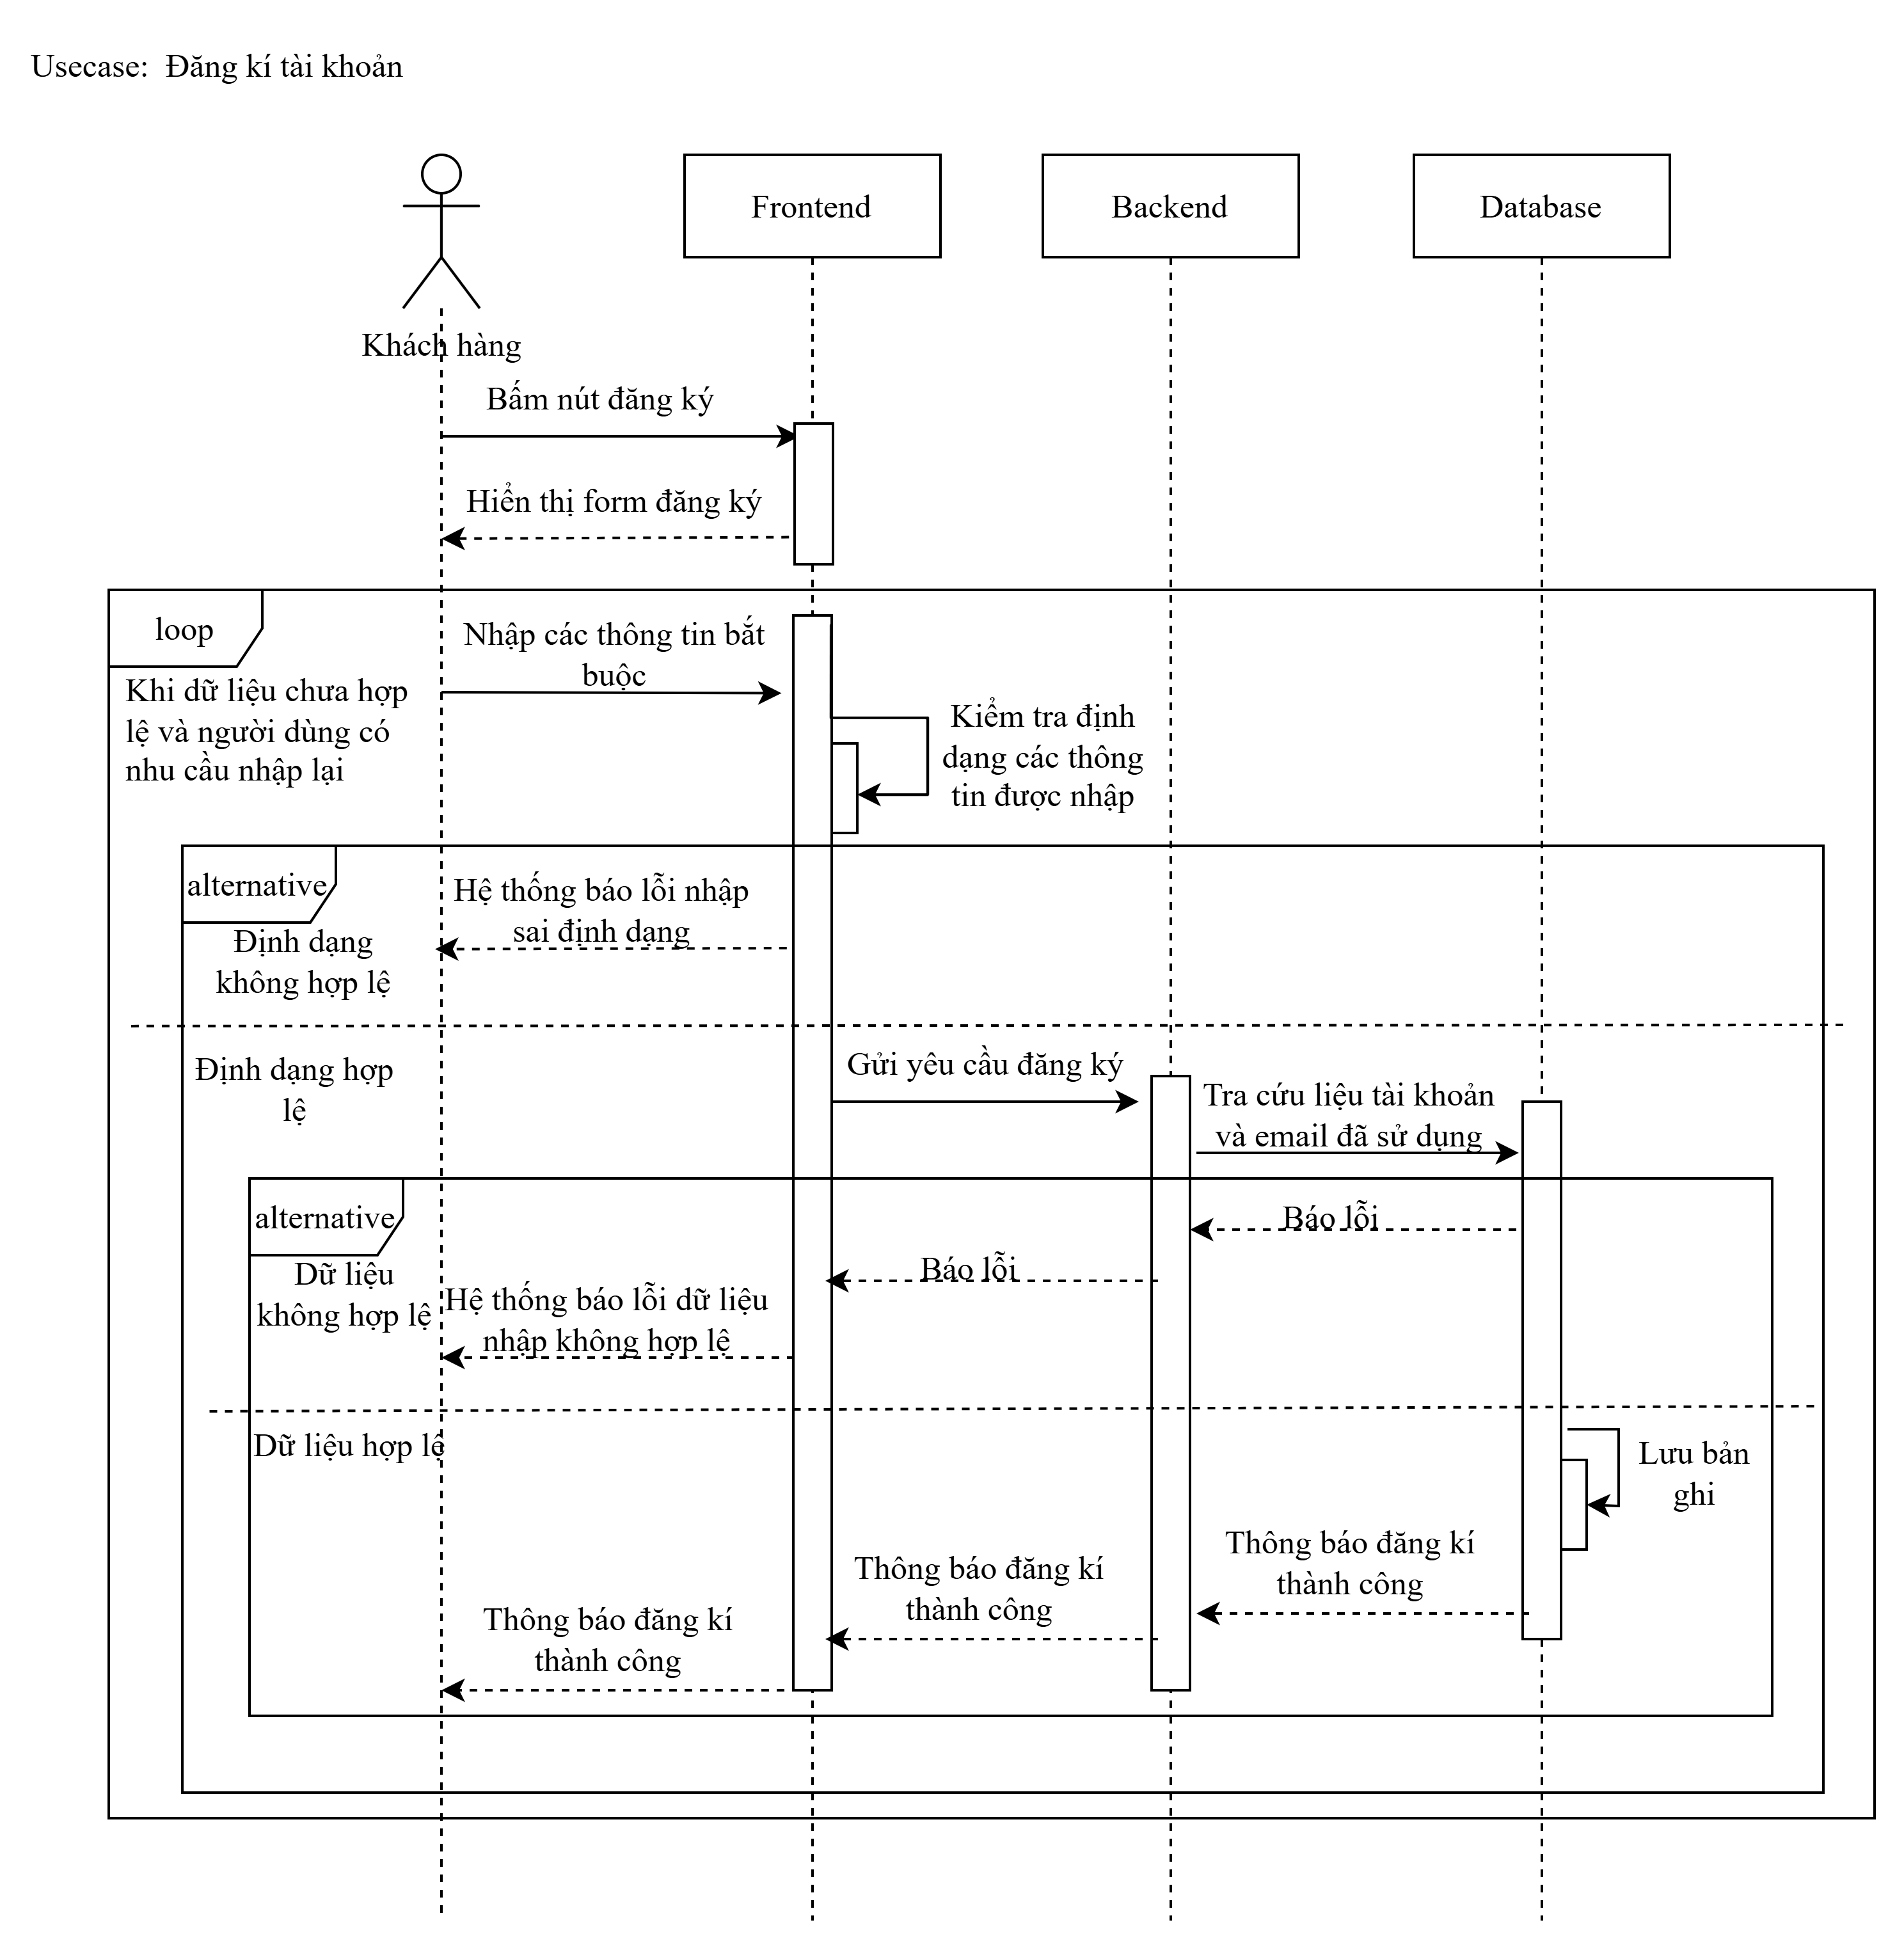
\includegraphics[width=0.9\linewidth]{images/chap3/sequence_diagram/register.png}
   \vspace{0.5cm} \caption{Sơ đồ tuần tự chức năng Đăng ký tài khoản}
    \label{fig:seq_register}
\end{figure}
Mô tả trình tự tương tác khi người dùng gửi yêu cầu đăng ký. Hệ thống kiểm tra sự tồn tại của email/tên đăng nhập trong cơ sở dữ liệu trước khi khởi tạo đối tượng tài khoản mới và phản hồi kết quả.

\begin{figure}[H]
    \centering
    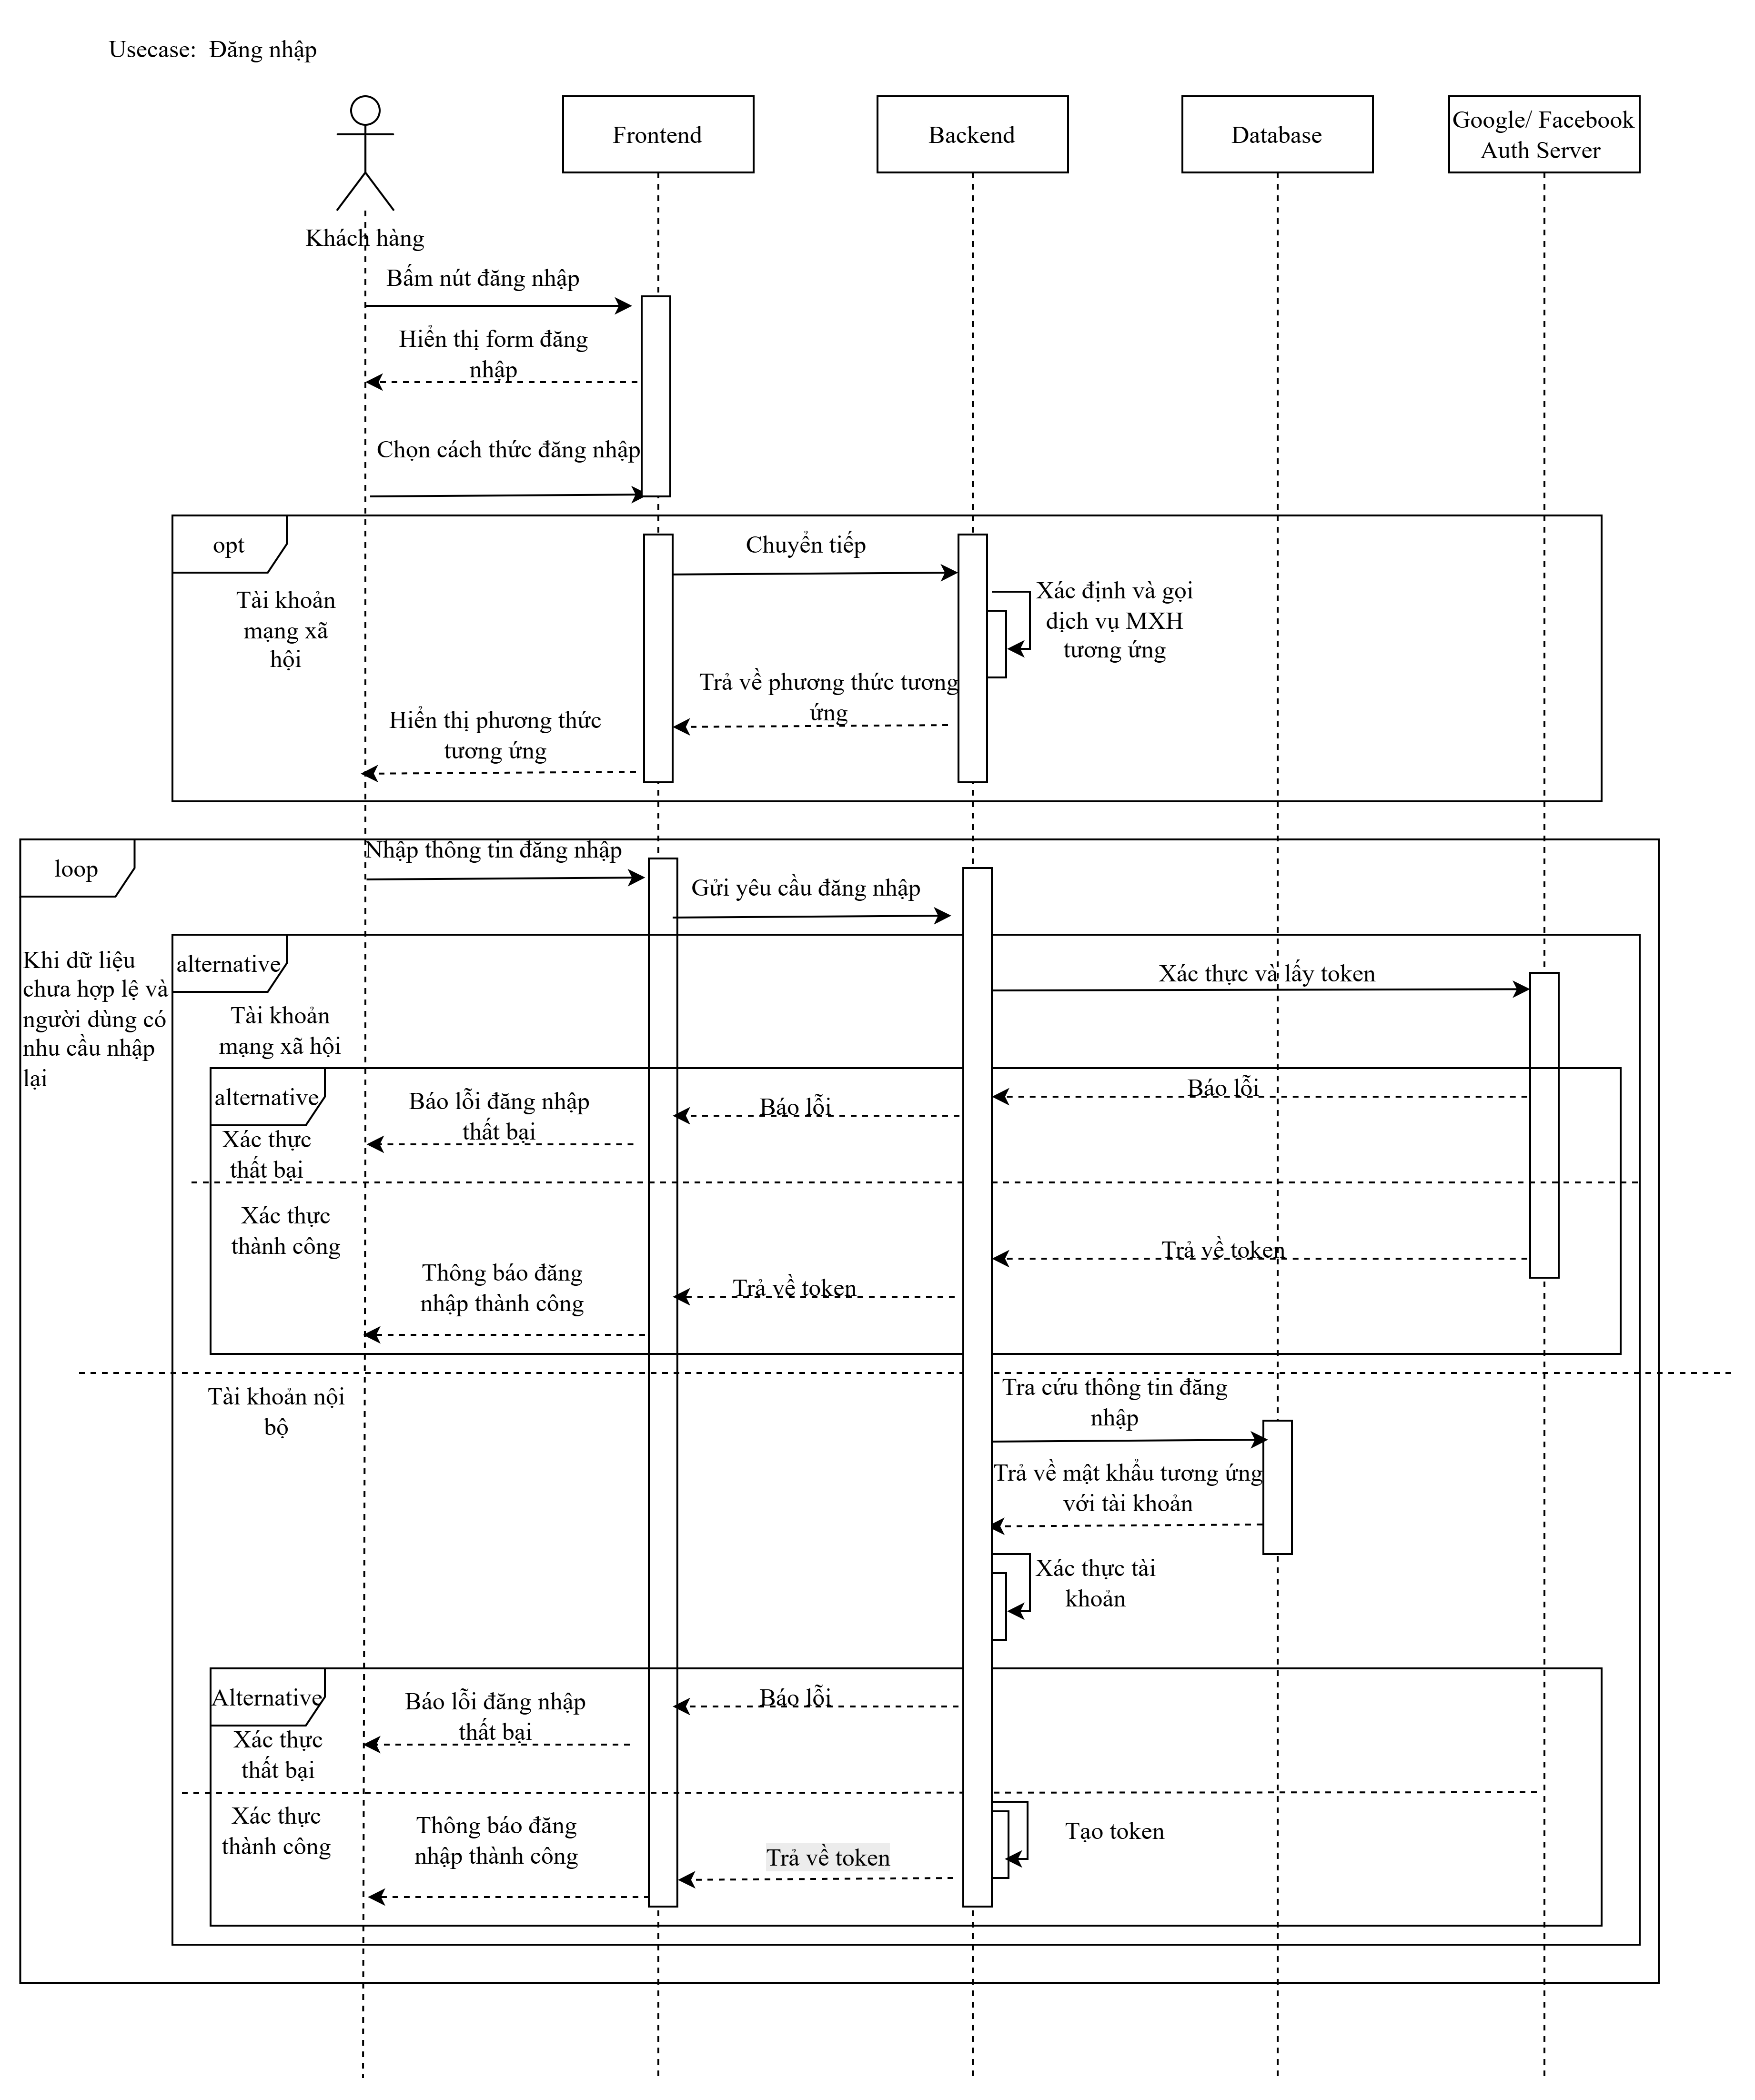
\includegraphics[width=0.9\linewidth]{images/chap3/sequence_diagram/login.png}
   \vspace{0.5cm} \caption{Sơ đồ tuần tự chức năng Đăng nhập}
    \label{fig:seq_login}
\end{figure}
Thể hiện luồng xác thực: Người dùng nhập thông tin, hệ thống đối chiếu dữ liệu mã hóa trong Database. Nếu khớp, hệ thống khởi tạo phiên làm việc (Session/Token) và chuyển hướng người dùng vào trang chủ.

\begin{figure}[H]
    \centering
    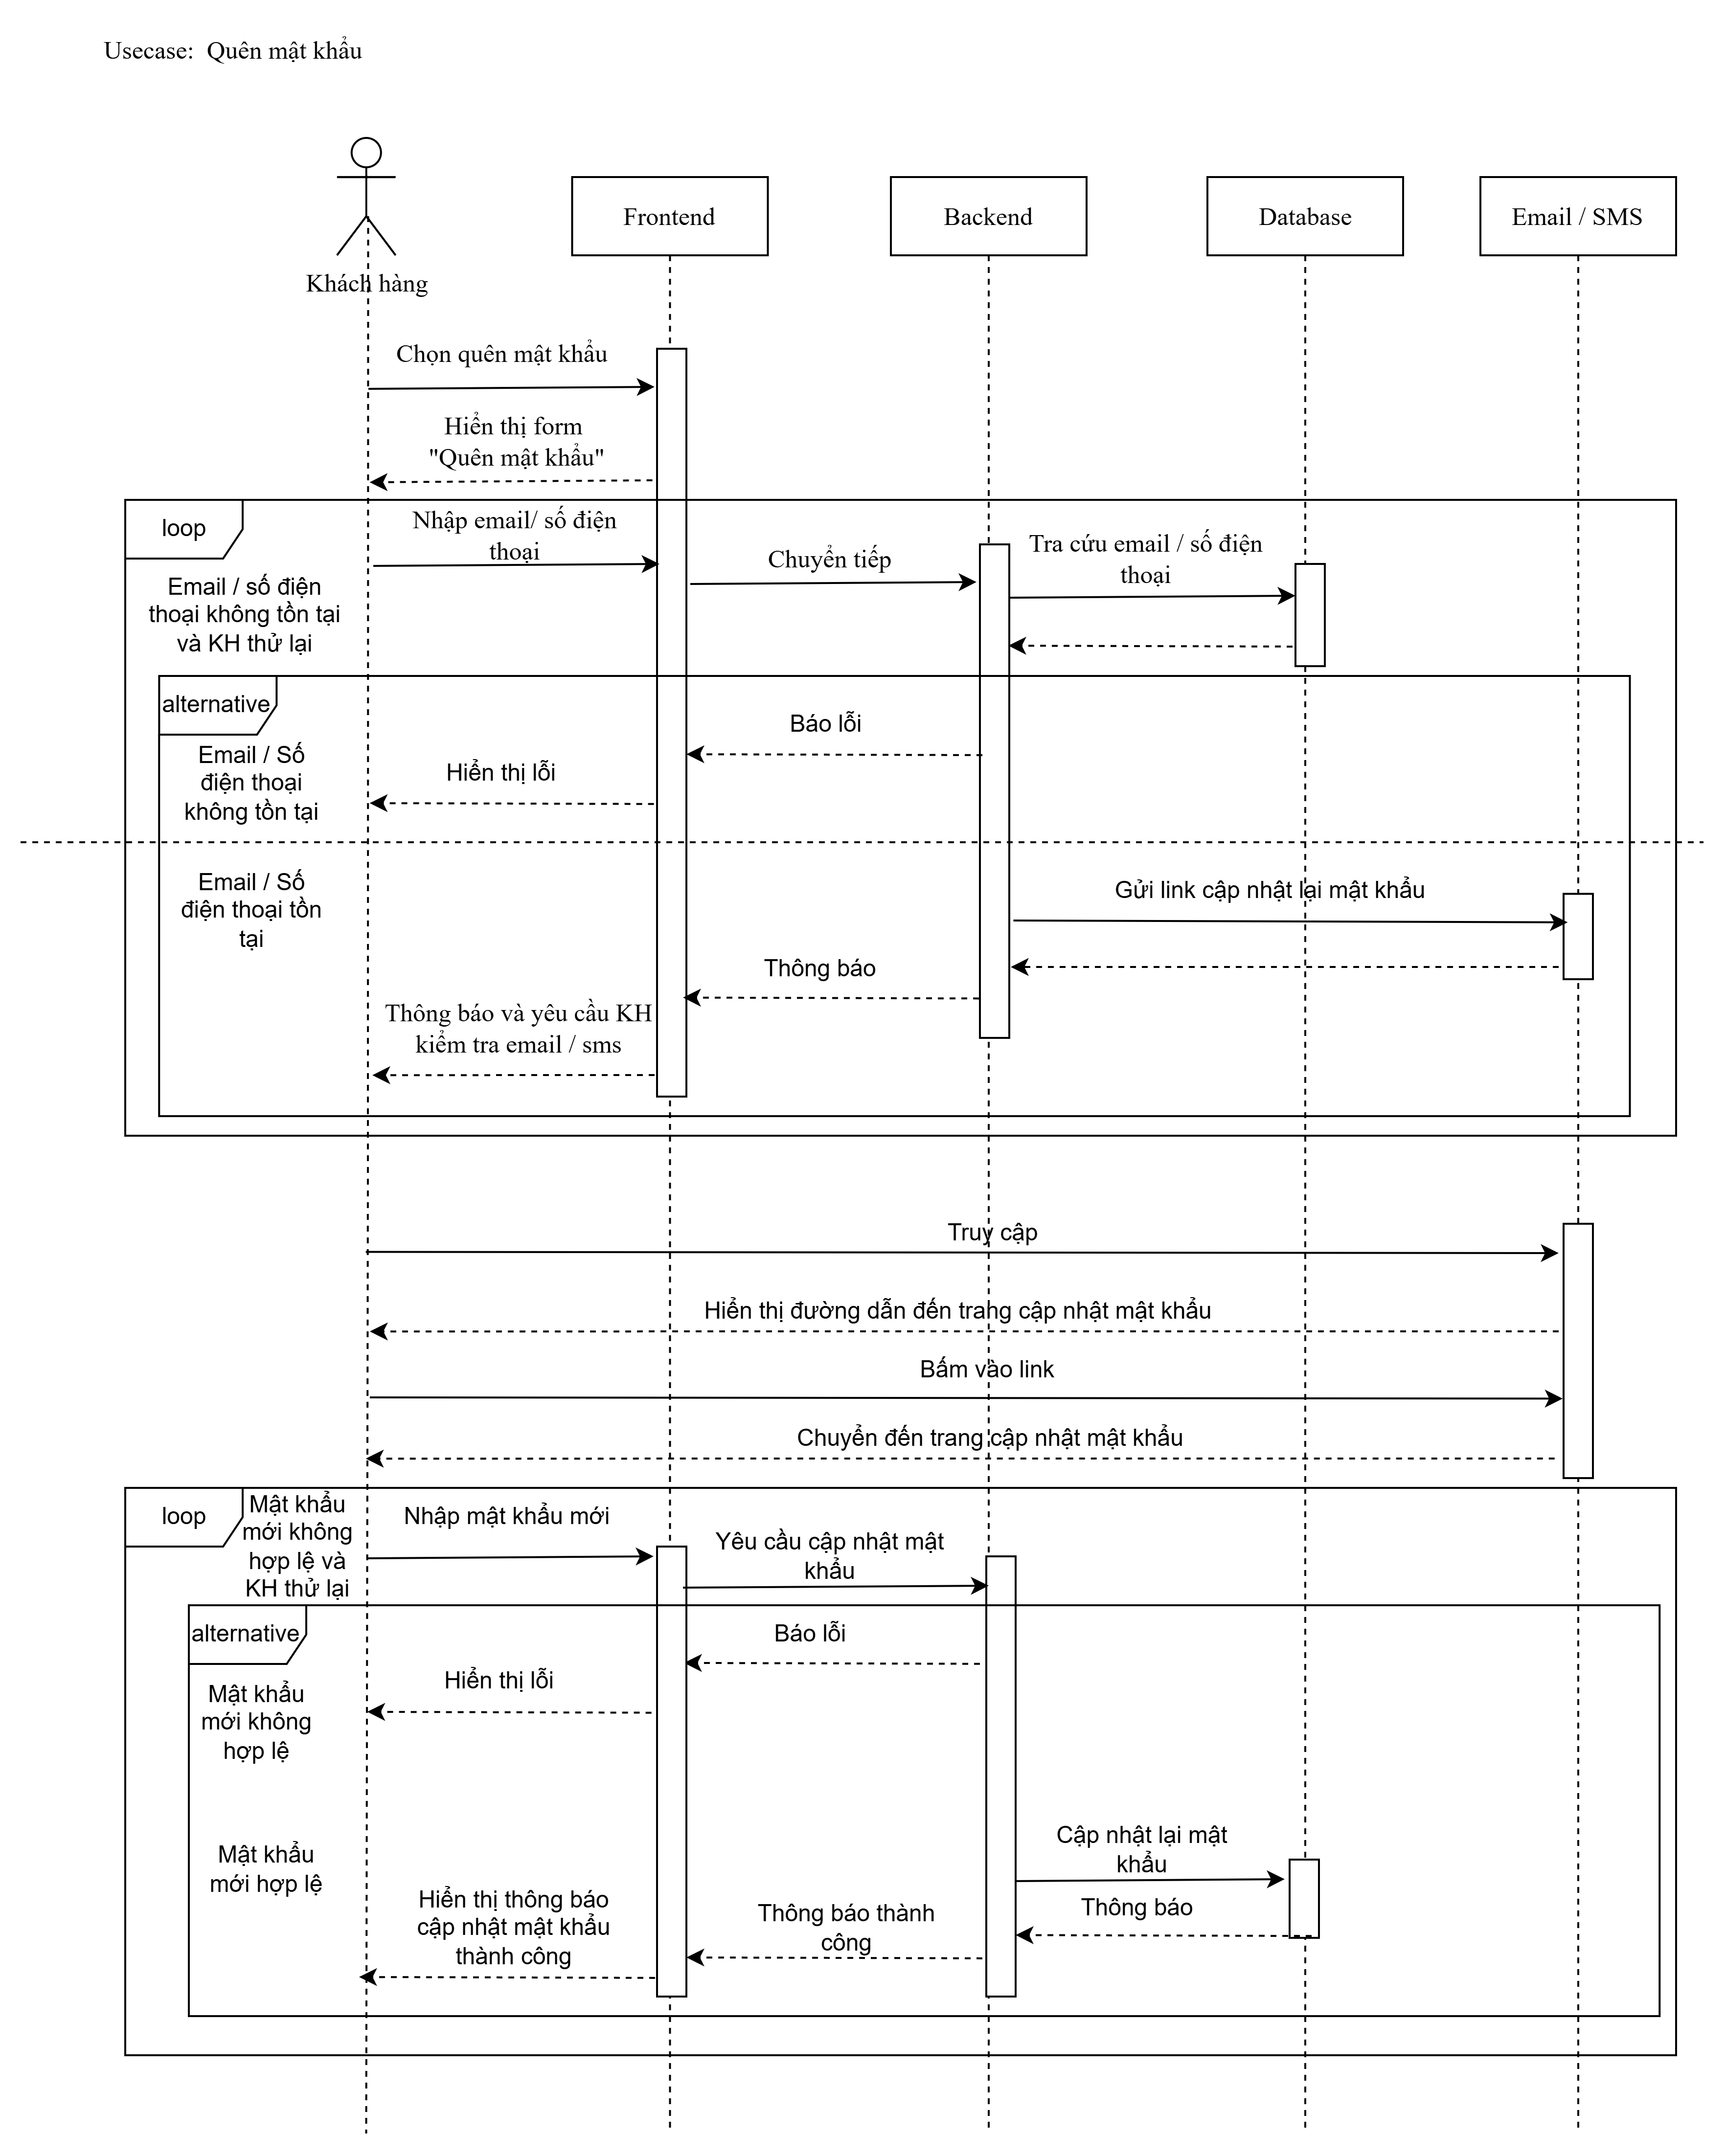
\includegraphics[width=0.9\linewidth]{images/chap3/sequence_diagram/forgot_password.png}
   \vspace{0.5cm} \caption{Sơ đồ tuần tự chức năng Quên mật khẩu}
    \label{fig:seq_forgot_pass}
\end{figure}
Mô tả quá trình tương tác để khôi phục tài khoản: Gửi yêu cầu xác thực qua email, kiểm tra mã xác nhận (OTP) và thực hiện cập nhật mật khẩu mới vào cơ sở dữ liệu.

\begin{figure}[H]
    \centering
    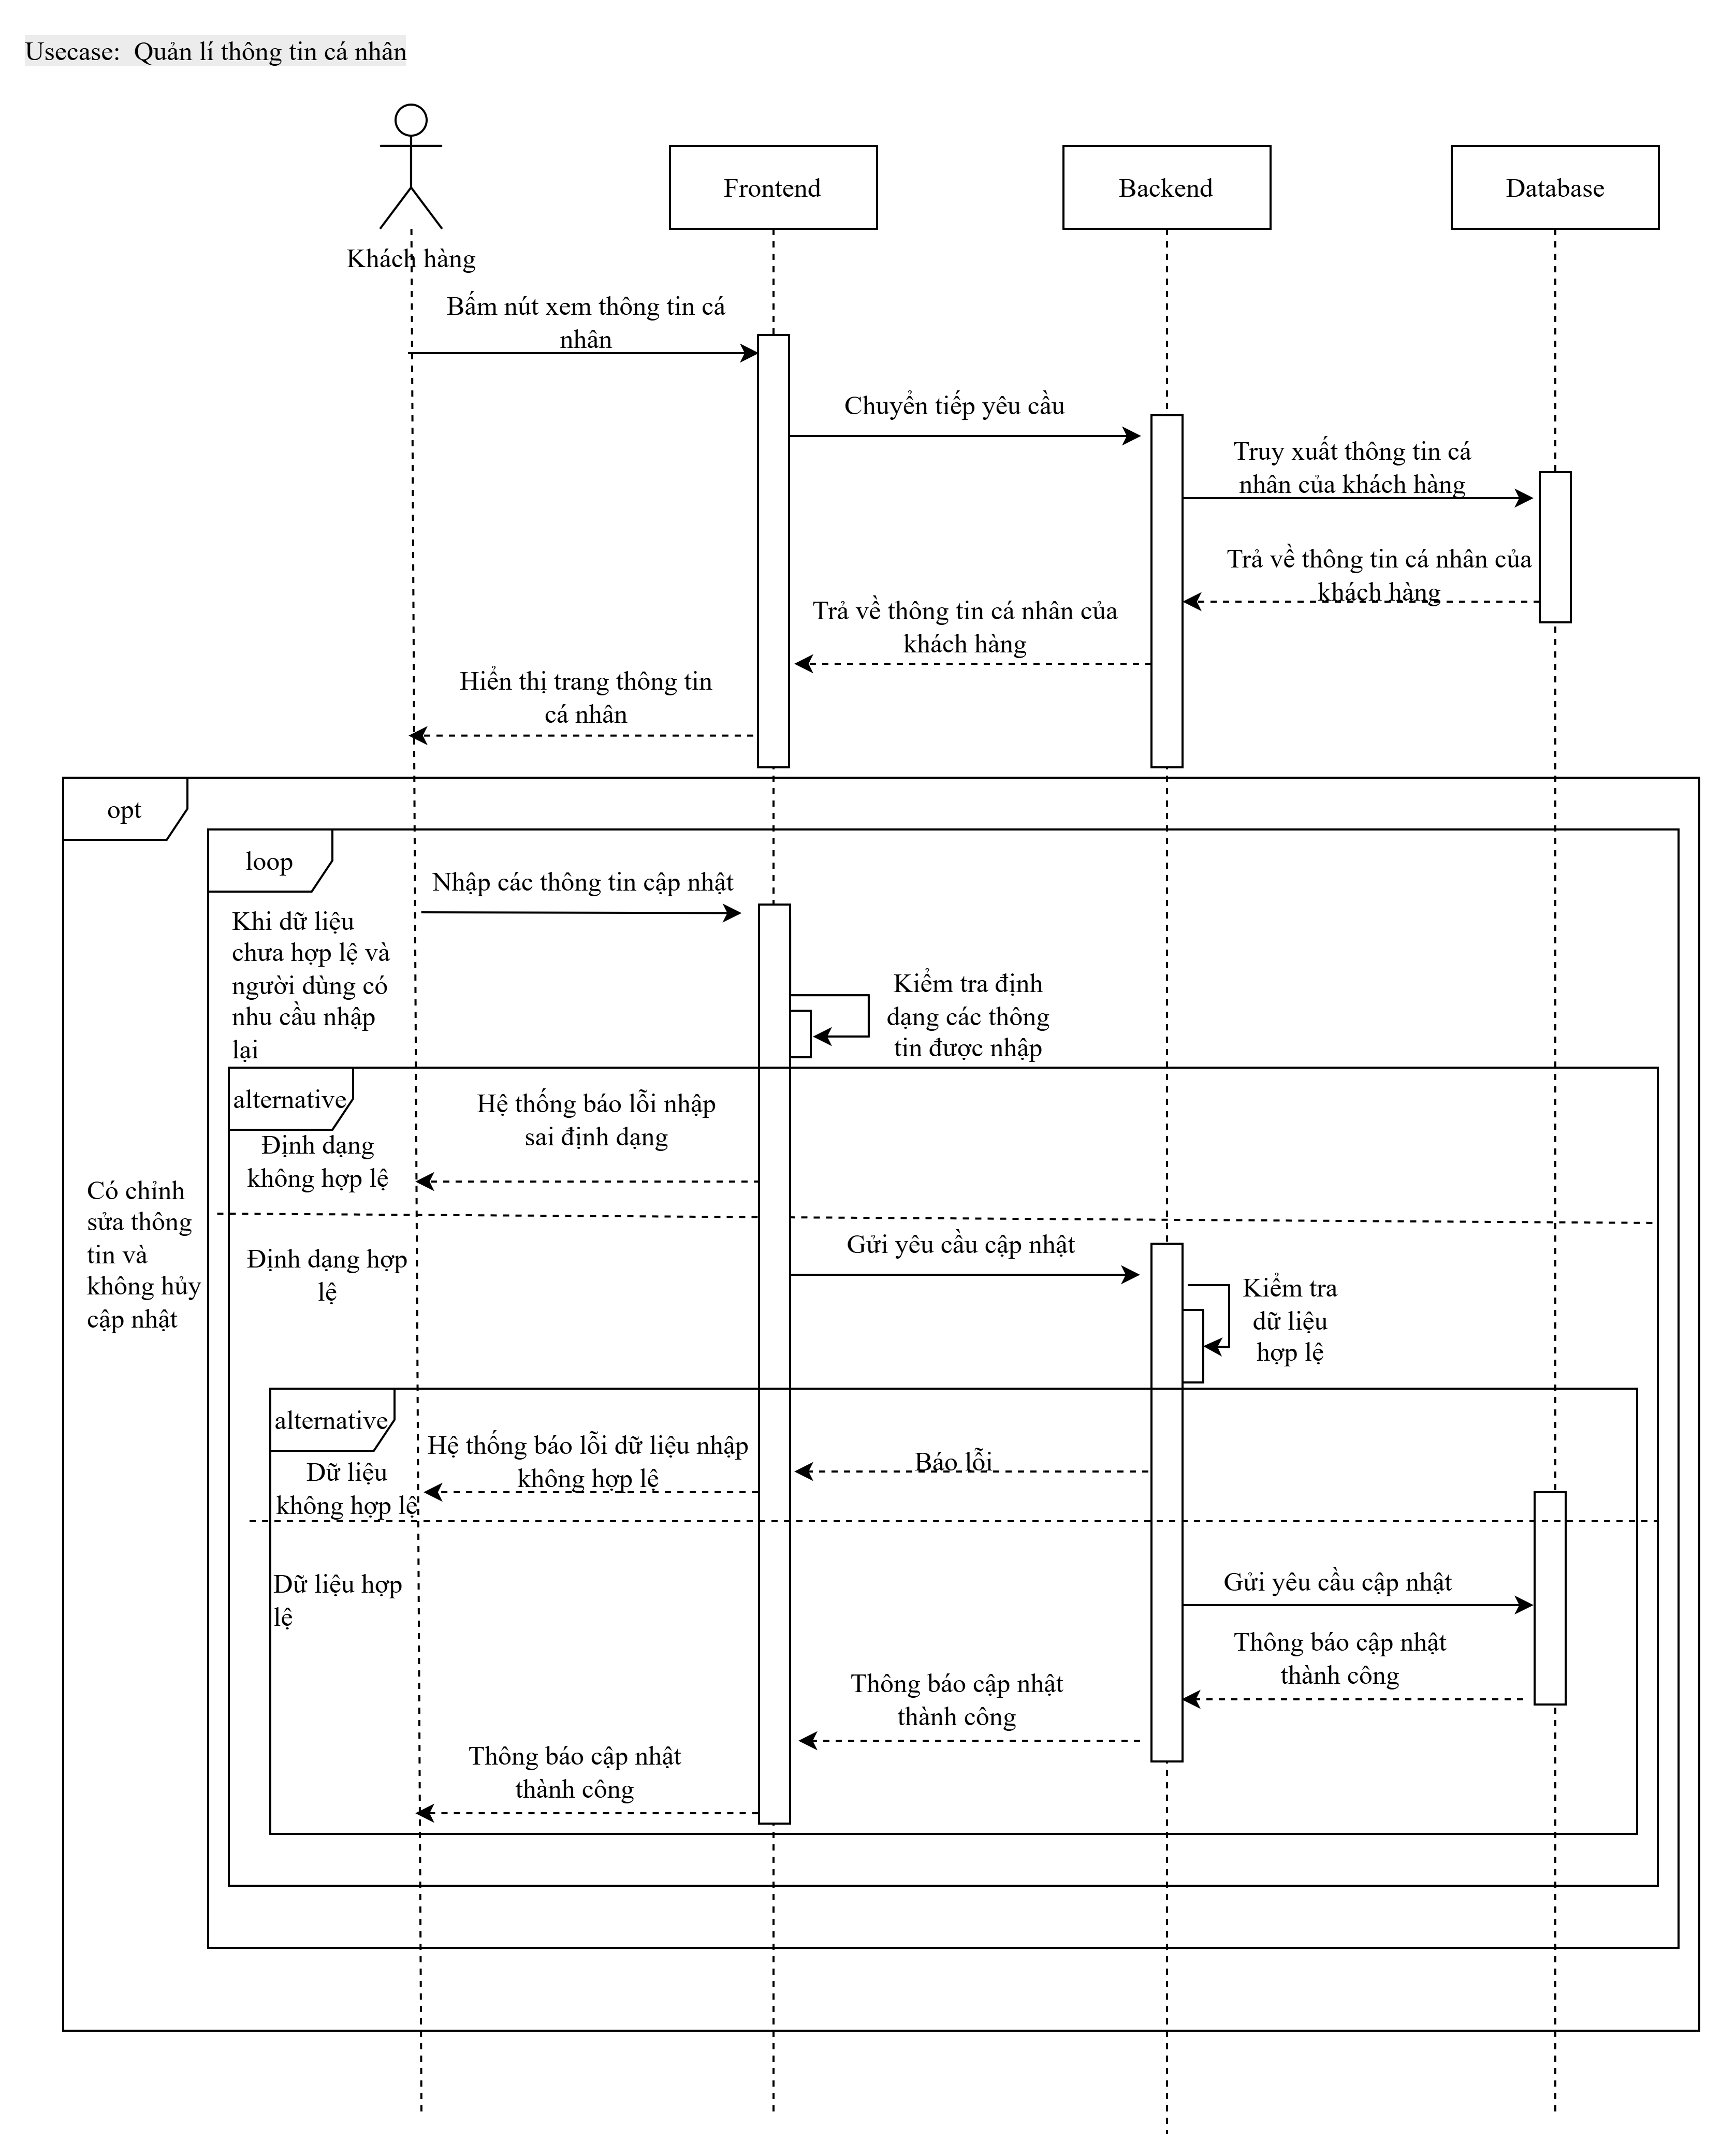
\includegraphics[width=0.9\linewidth]{images/chap3/sequence_diagram/manage_personal_information.png}
   \vspace{0.5cm} \caption{Sơ đồ tuần tự Quản lý thông tin cá nhân}
    \label{fig:seq_manage_info}
\end{figure}
Người dùng yêu cầu xem hoặc sửa đổi thông tin. Hệ thống truy xuất dữ liệu hiện tại để hiển thị, sau đó nhận dữ liệu mới, thực hiện validation và cập nhật lại vào hệ thống lưu trữ.

% --- NHÓM 2: QUY TRÌNH MUA SẮM (SHOPPING FLOW) ---

\begin{figure}[H]
    \centering
    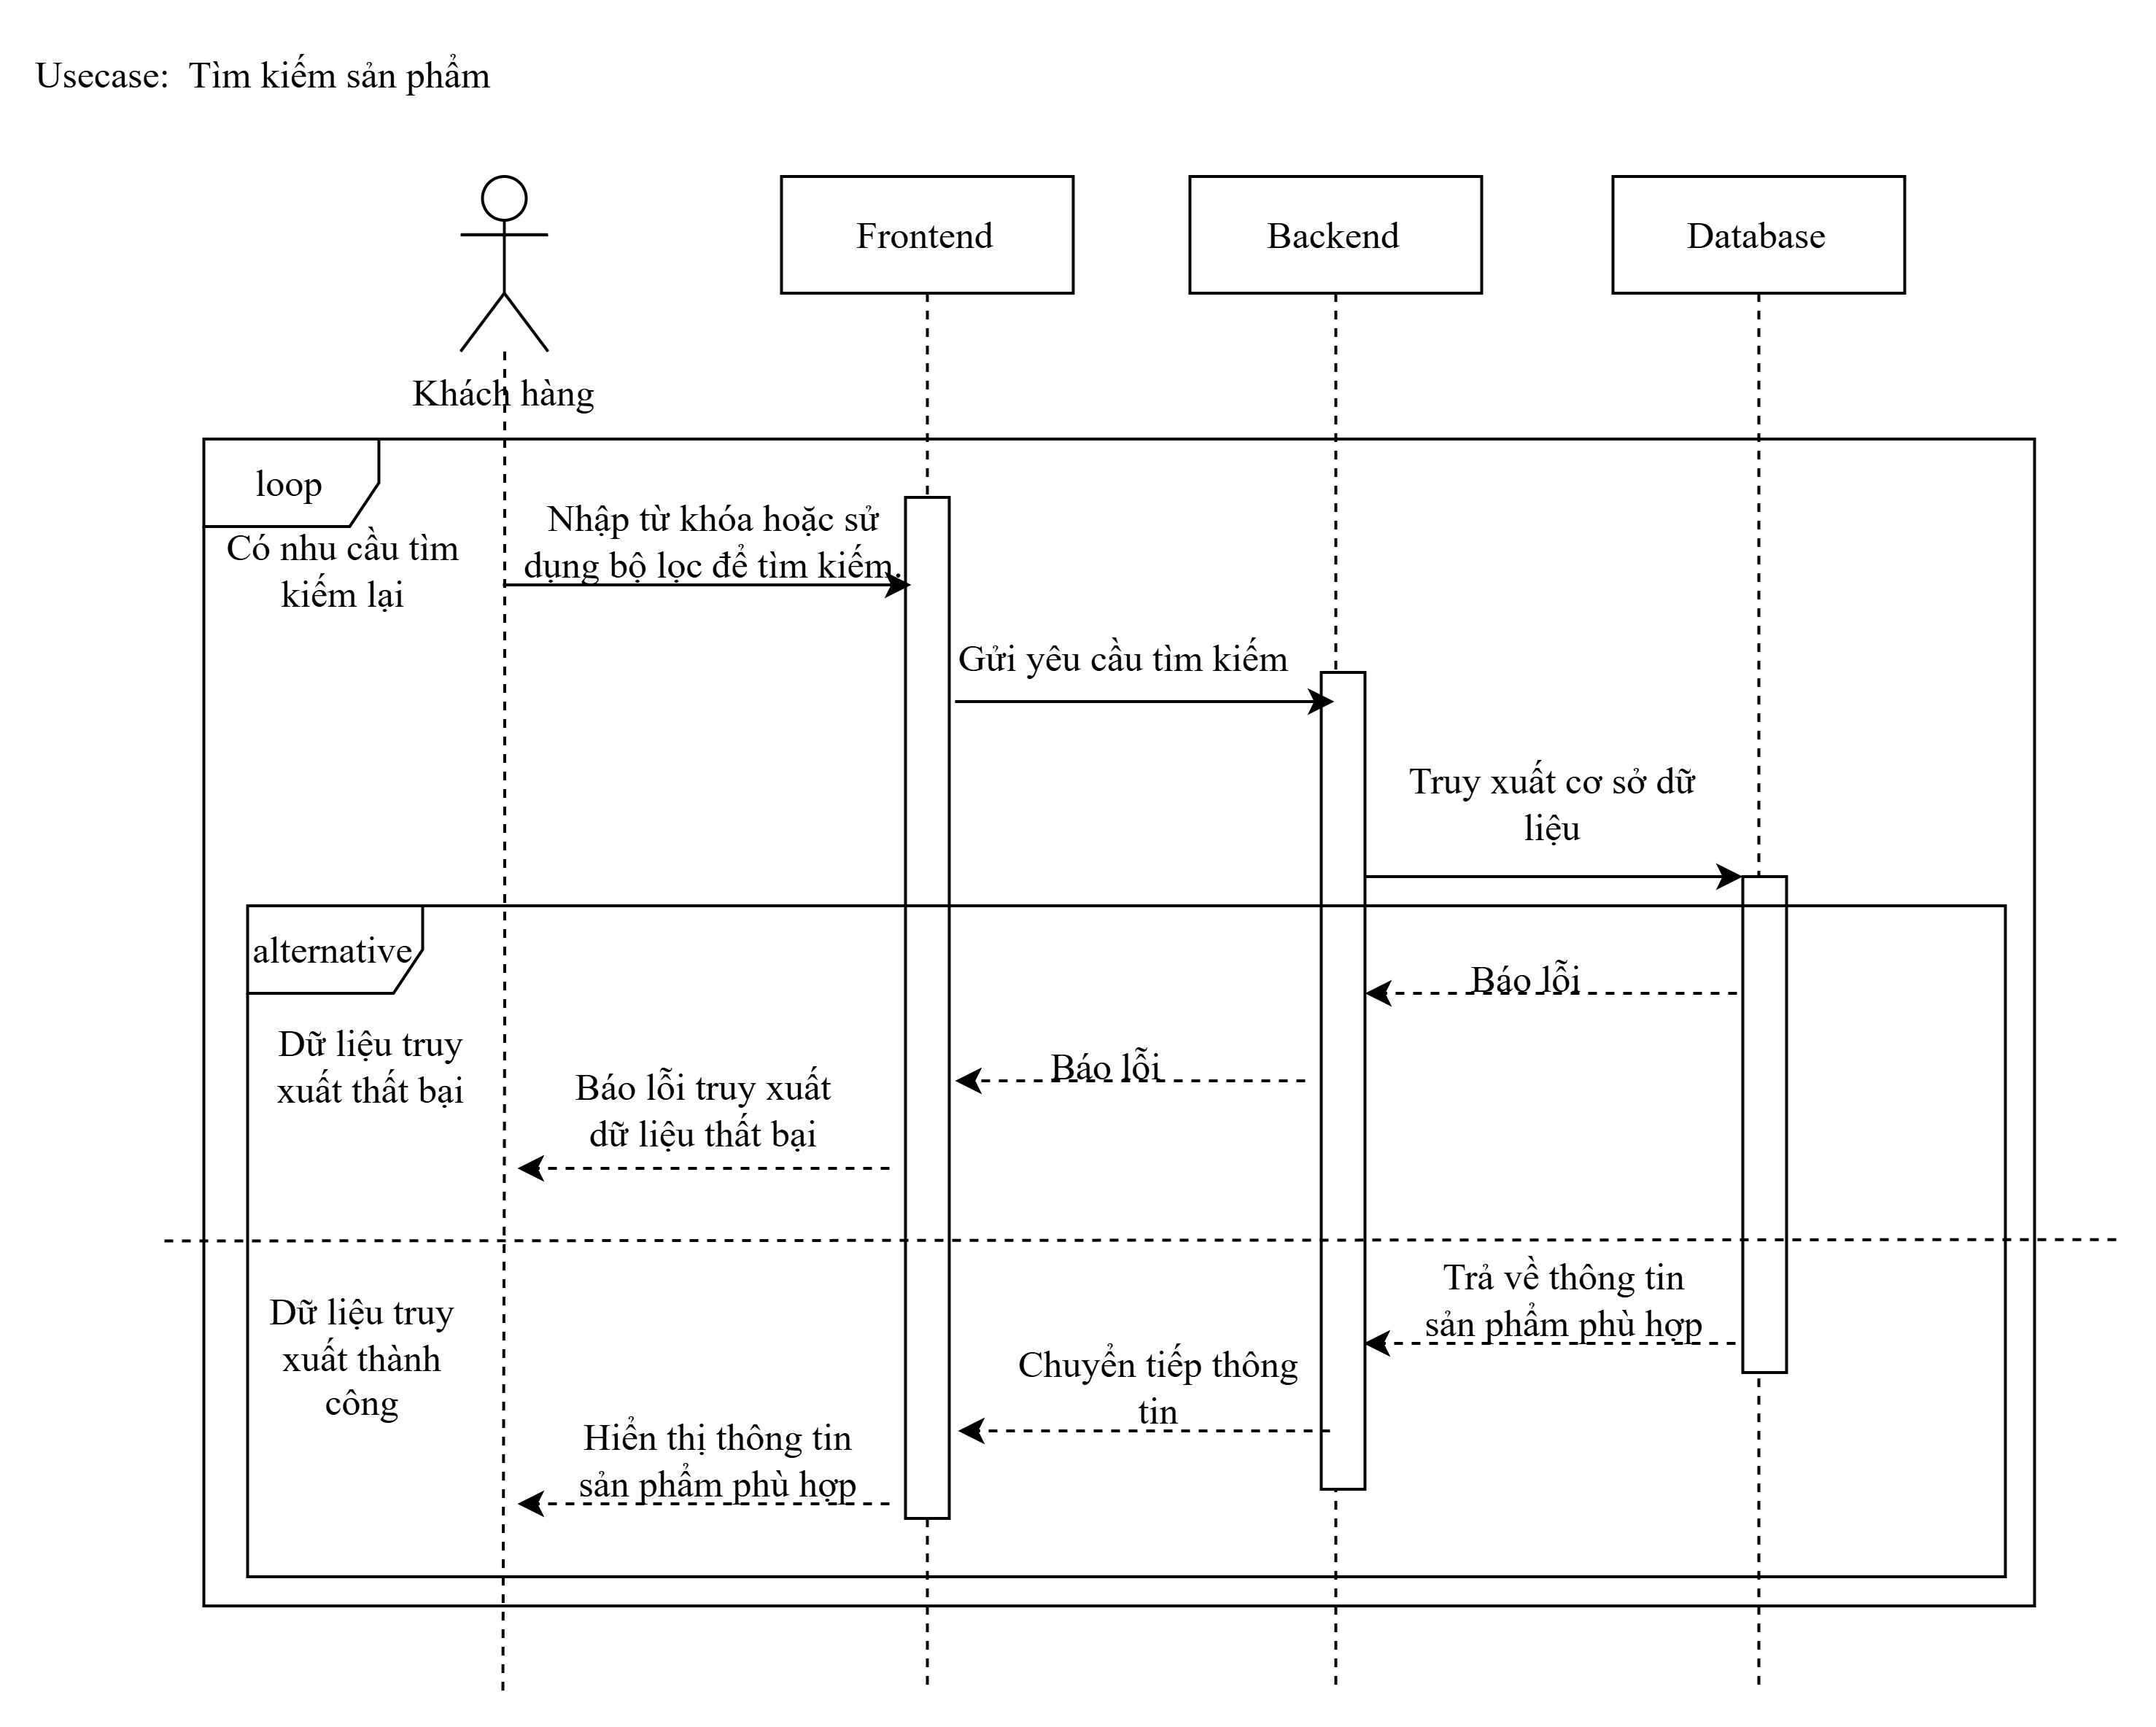
\includegraphics[width=1.0\linewidth]{images/chap3/sequence_diagram/find_product.png}
   \vspace{0.5cm} \caption{Sơ đồ tuần tự Tìm kiếm sản phẩm}
    \label{fig:seq_find_product}
\end{figure}
Người dùng gửi từ khóa hoặc bộ lọc. Controller xử lý yêu cầu, truy vấn danh sách sản phẩm từ Database thỏa mãn điều kiện và trả về danh sách kết quả hiển thị cho người dùng.

\begin{figure}[H]
    \centering
    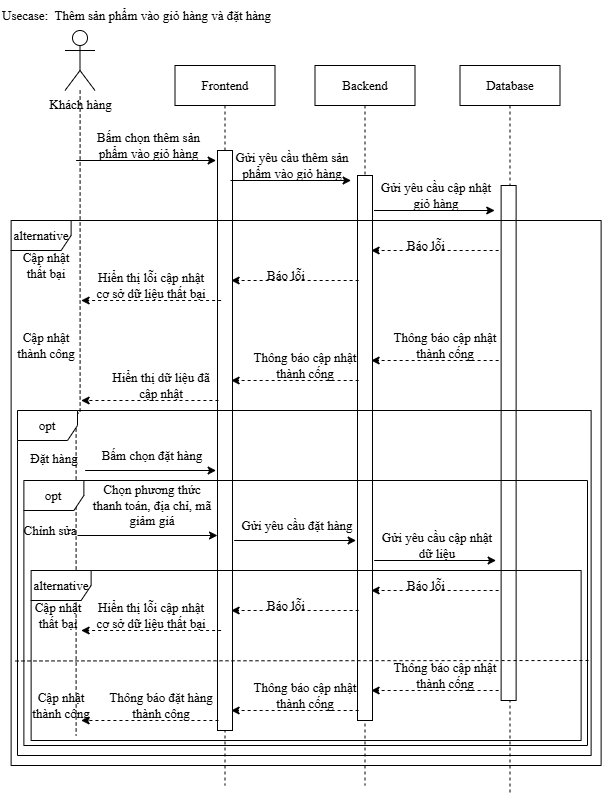
\includegraphics[width=1.0\linewidth]{images/chap3/sequence_diagram/add_to_cart_and_checkout.png}
   \vspace{0.5cm} \caption{Sơ đồ tuần tự Thêm vào giỏ và Đặt hàng}
    \label{fig:seq_cart_checkout}
\end{figure}
Sơ đồ phức tạp mô tả chuỗi hành động: Kiểm tra tồn kho khi thêm vào giỏ -> Cập nhật giỏ hàng -> Khởi tạo đơn hàng (Order) -> Lưu chi tiết đơn hàng (Order Details) và xác nhận đặt hàng thành công.

\begin{figure}[H]
    \centering
    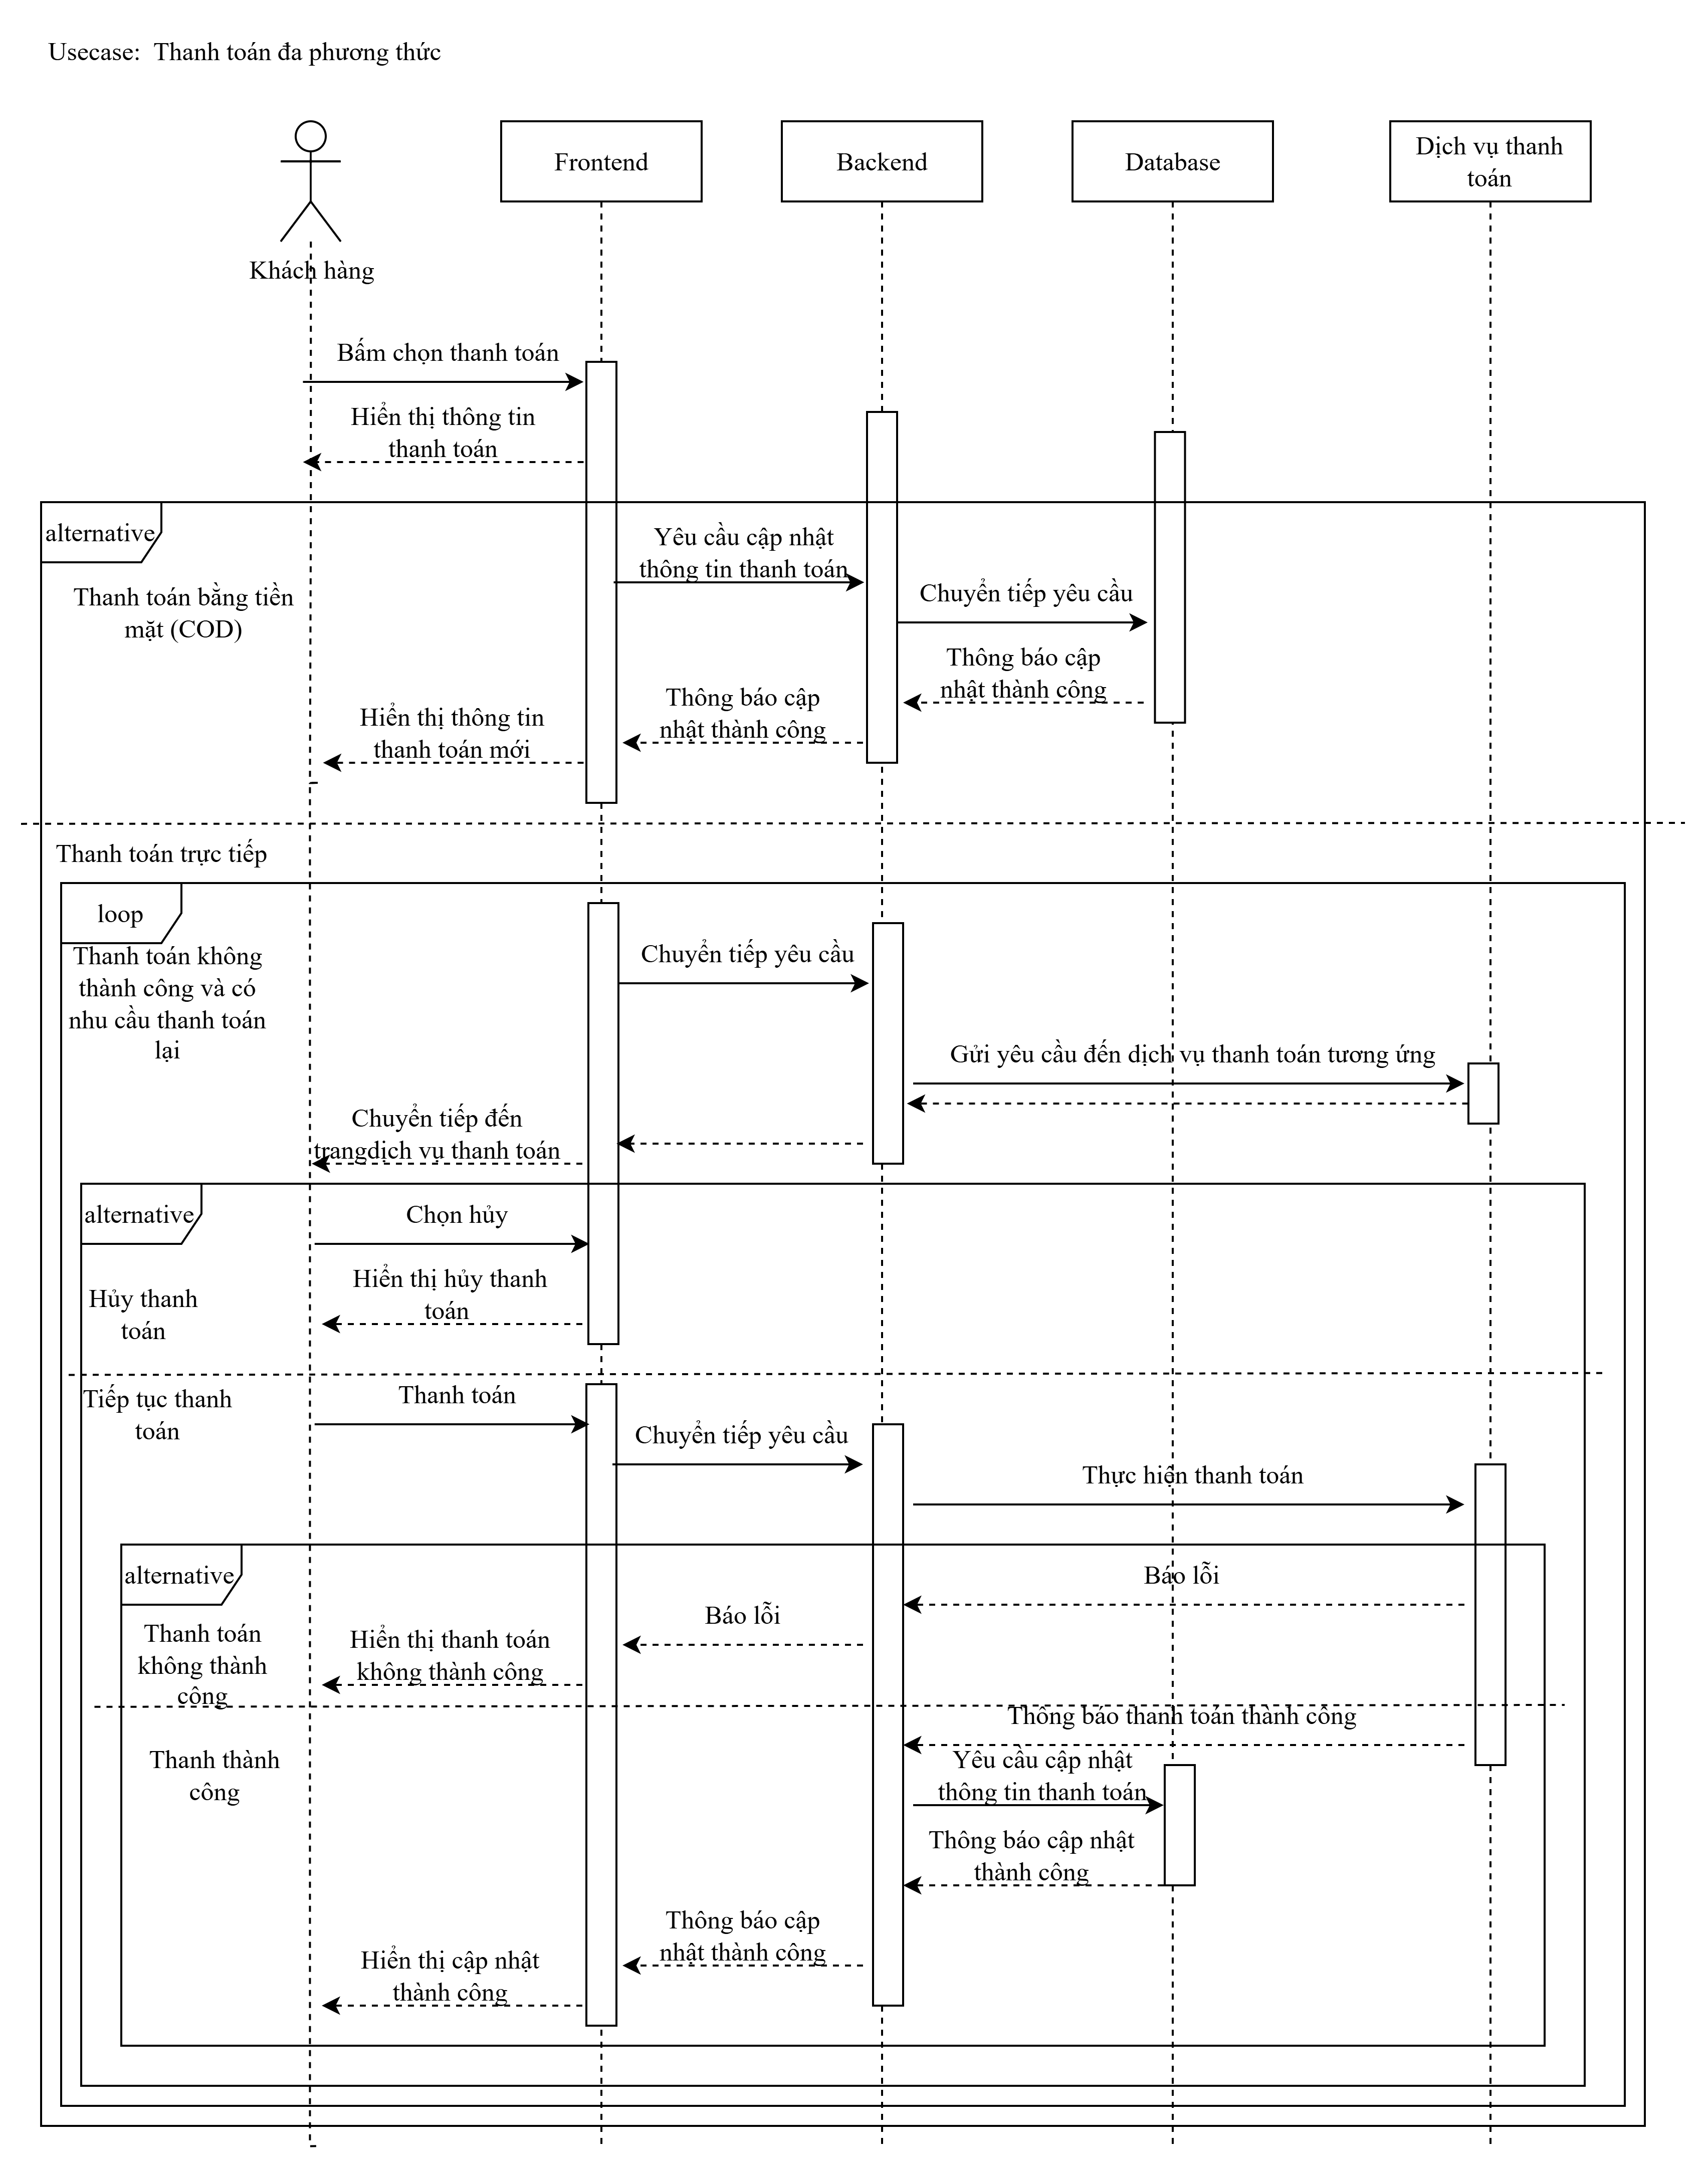
\includegraphics[width=0.9\linewidth]{images/chap3/sequence_diagram/multiple_payment_method.png}
   \vspace{0.5cm} \caption{Sơ đồ tuần tự Thanh toán đa phương thức}
    \label{fig:seq_payment}
\end{figure}
Mô tả việc người dùng chọn phương thức thanh toán. Hệ thống có thể tương tác với cổng thanh toán bên ngoài (API) hoặc xử lý thanh toán nội bộ, sau đó cập nhật trạng thái thanh toán cho đơn hàng.

% --- NHÓM 3: QUẢN LÝ ĐƠN HÀNG CỦA NGƯỜI DÙNG (USER ORDER MANAGEMENT) ---

\begin{figure}[H]
    \centering
    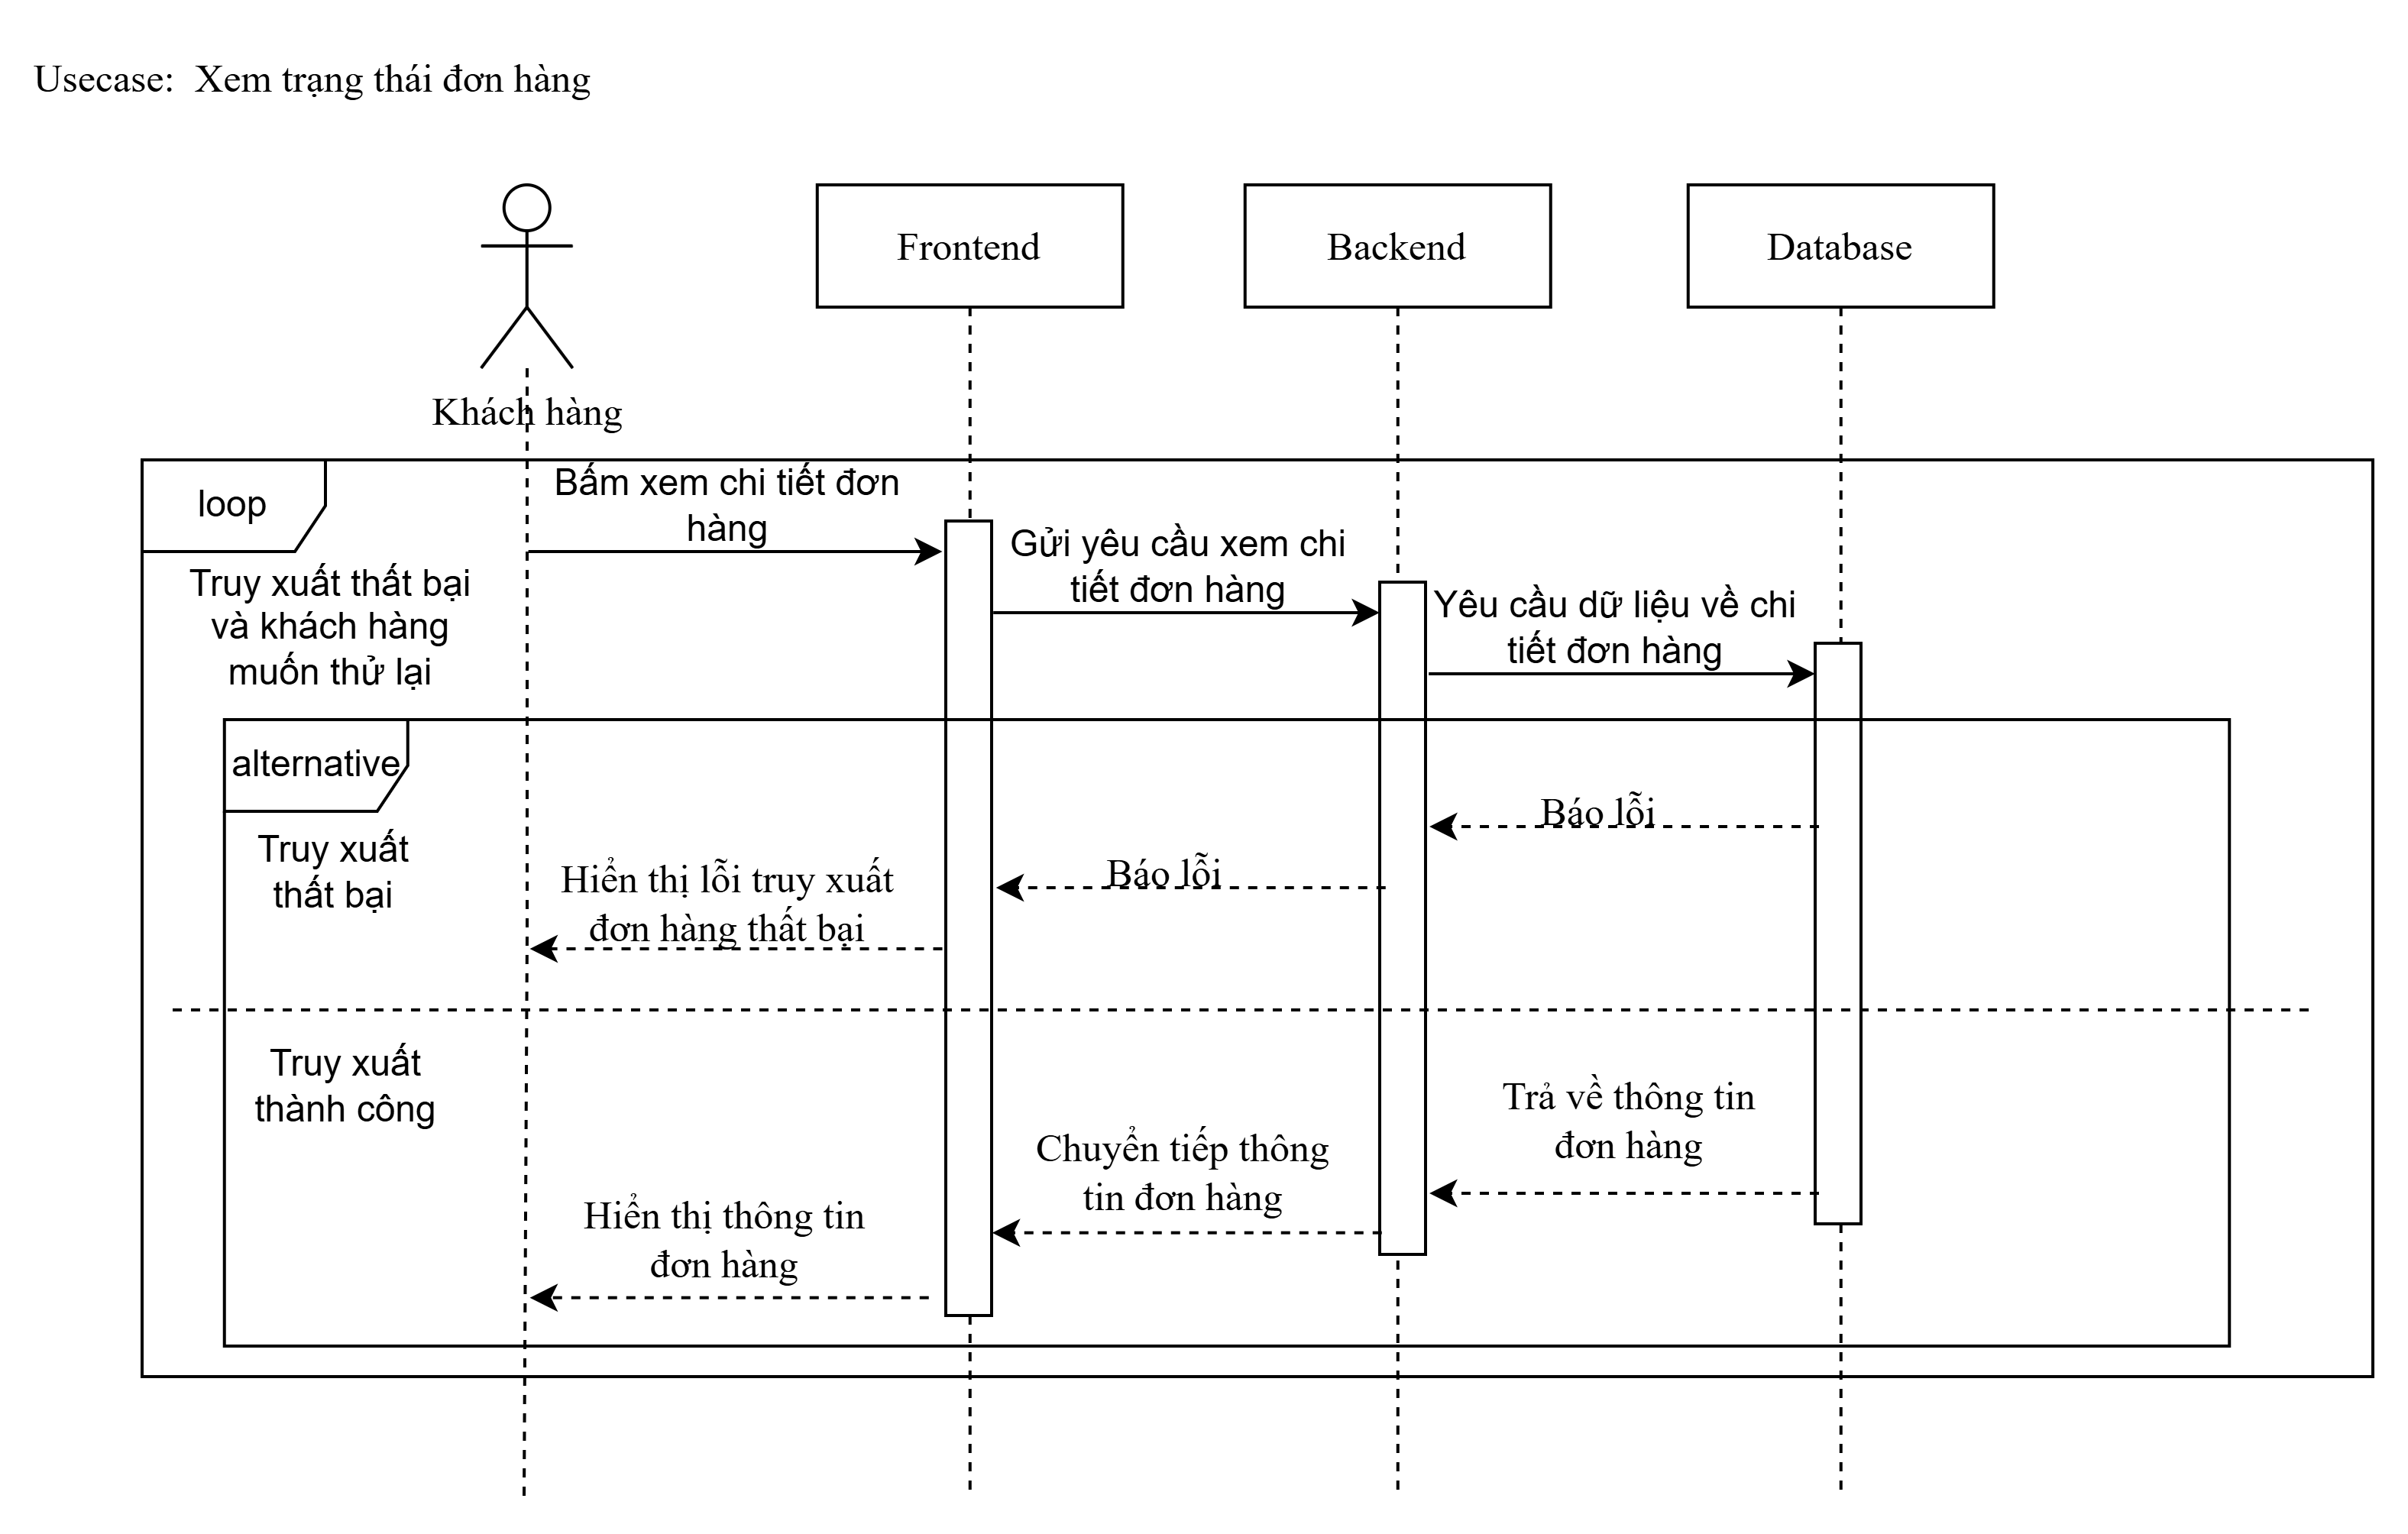
\includegraphics[width=0.9\linewidth]{images/chap3/sequence_diagram/view_order_status.png}
   \vspace{0.5cm} \caption{Sơ đồ tuần tự Xem trạng thái đơn hàng}
    \label{fig:seq_view_order}
\end{figure}
Người dùng gửi yêu cầu xem chi tiết đơn hàng. Hệ thống truy xuất thông tin từ bảng Order và OrderDetails, trả về trạng thái hiện tại (ví dụ: Đang giao, Đã hoàn thành) cho giao diện người dùng.

\begin{figure}[H]
    \centering
    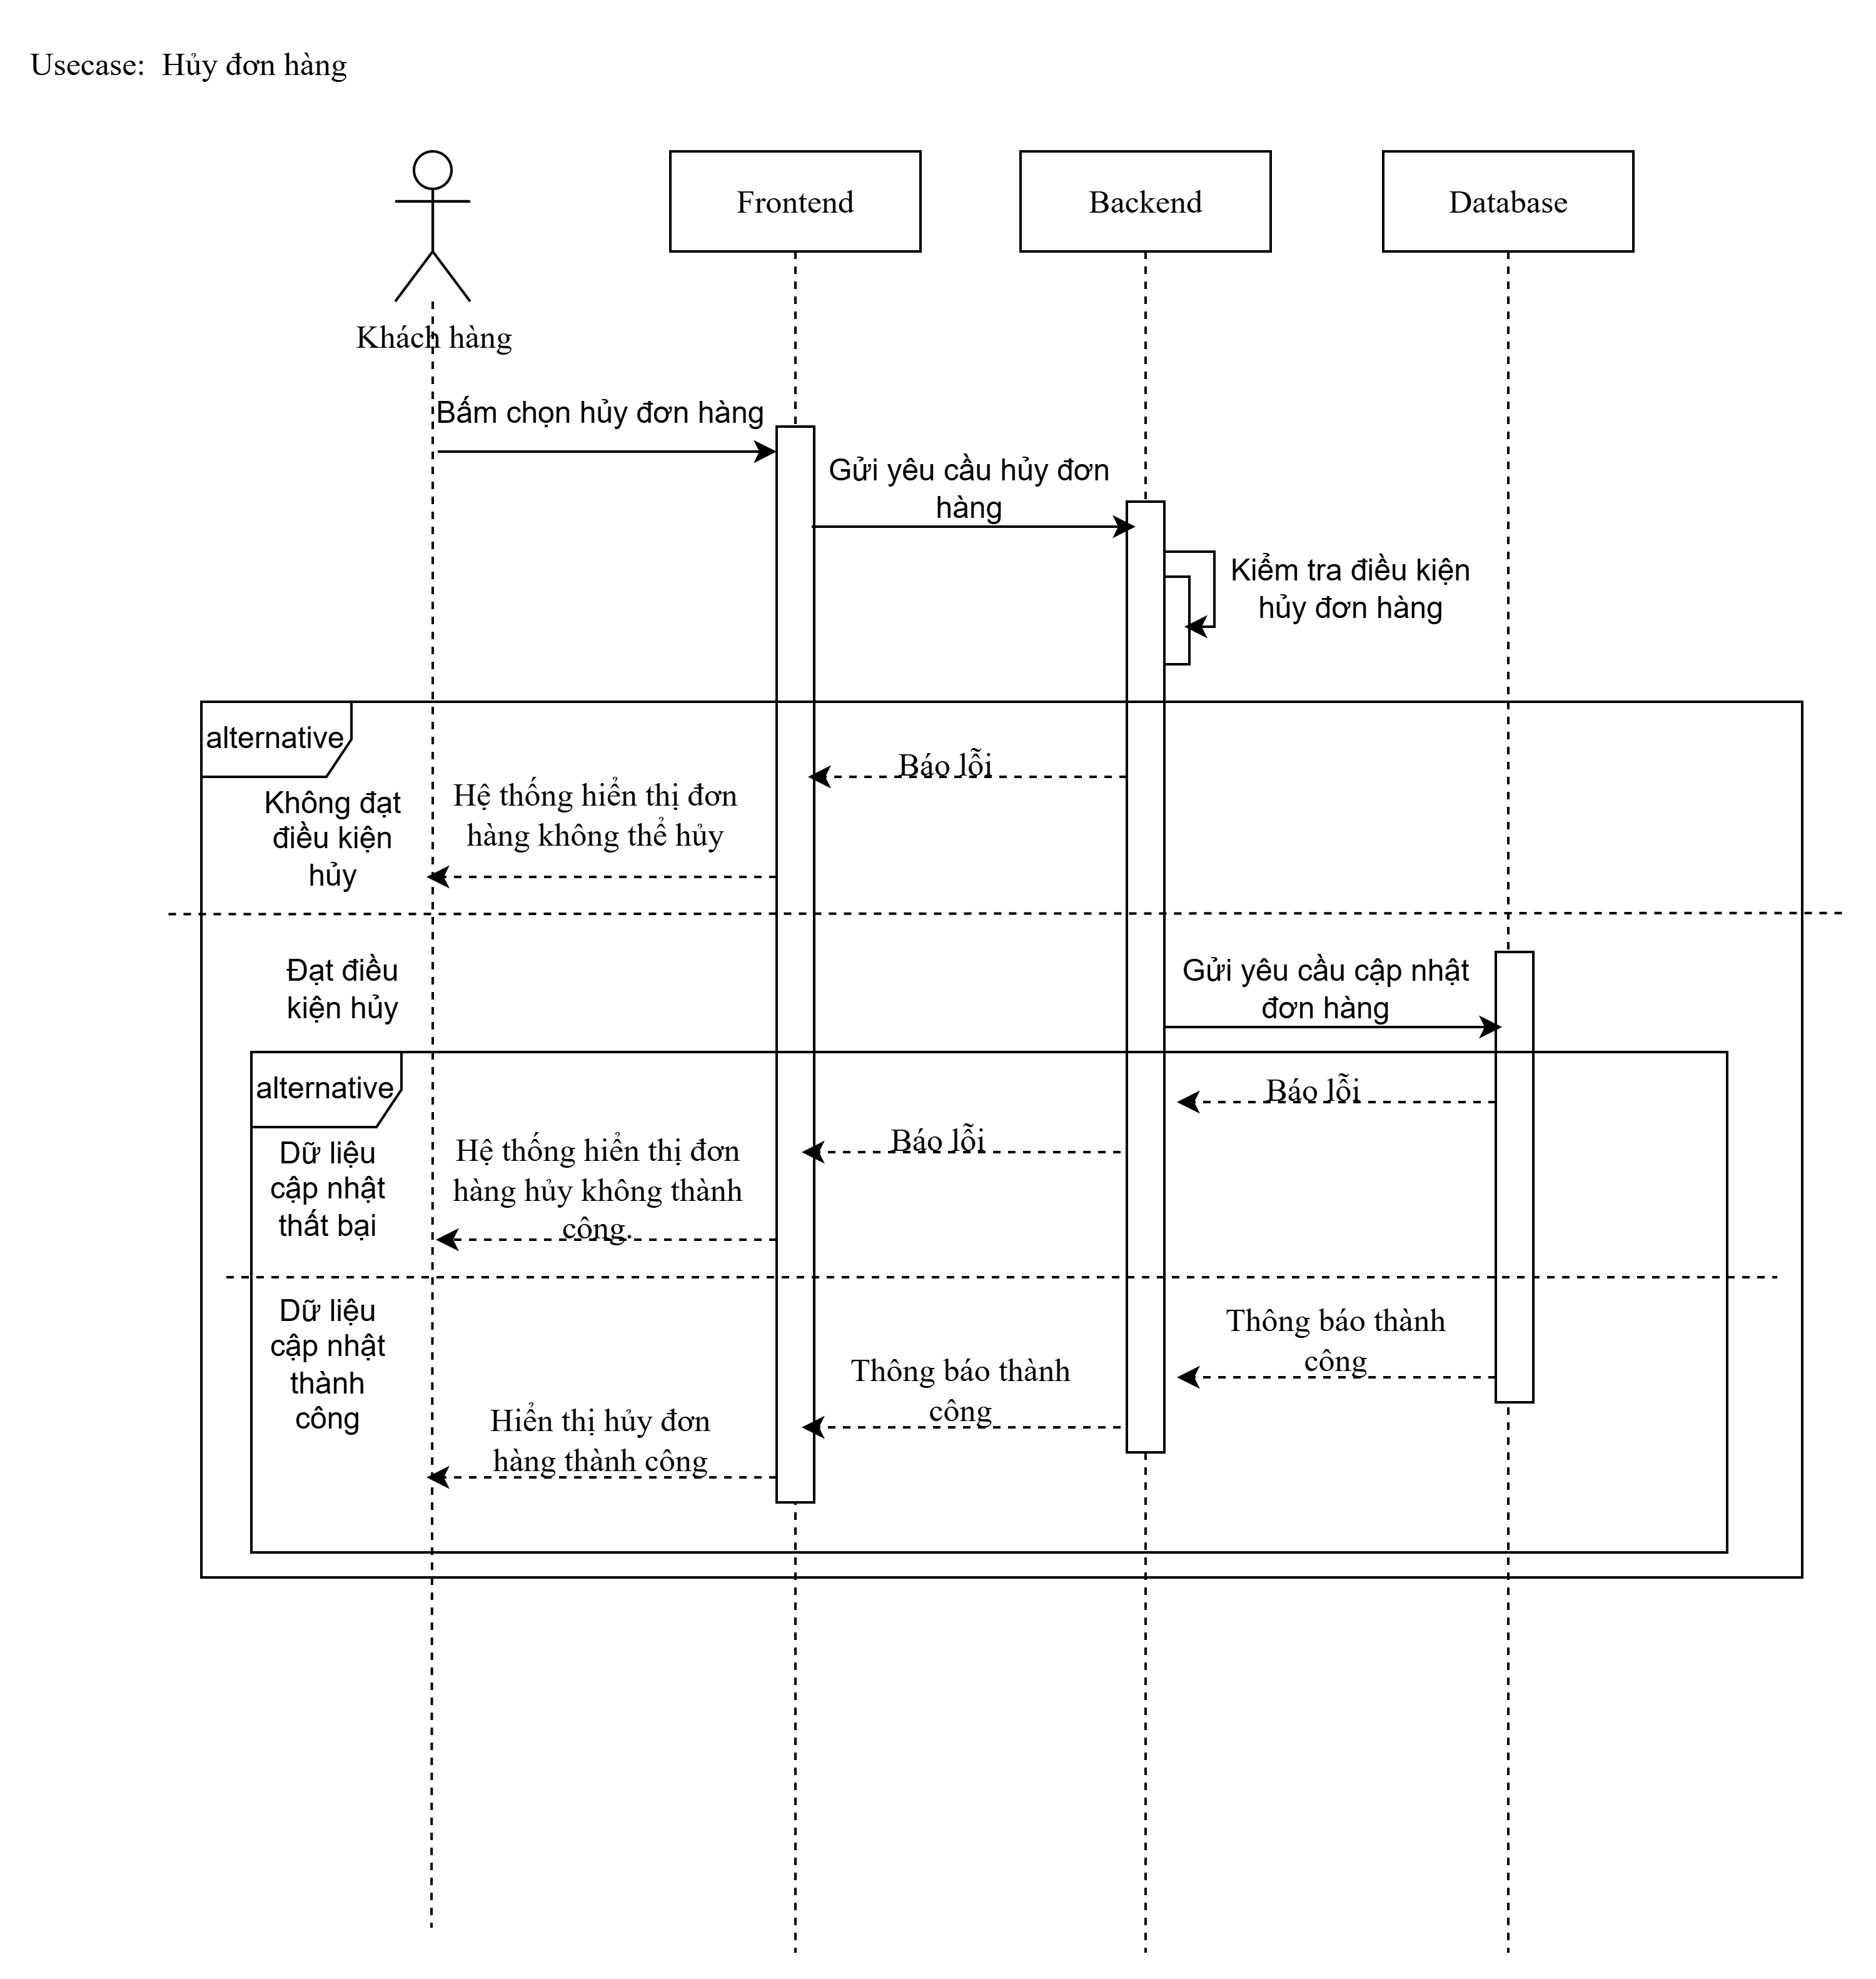
\includegraphics[width=0.9\linewidth]{images/chap3/sequence_diagram/cancel_order.png}
   \vspace{0.5cm} \caption{Sơ đồ tuần tự Hủy đơn hàng (Người dùng)}
    \label{fig:seq_cancel_order}
\end{figure}
Hệ thống kiểm tra điều kiện hủy (ví dụ: đơn chưa giao). Nếu hợp lệ, hệ thống cập nhật trạng thái đơn hàng thành "Cancelled", hoàn lại tồn kho (nếu cần) và thông báo thành công.

\begin{figure}[H]
    \centering
    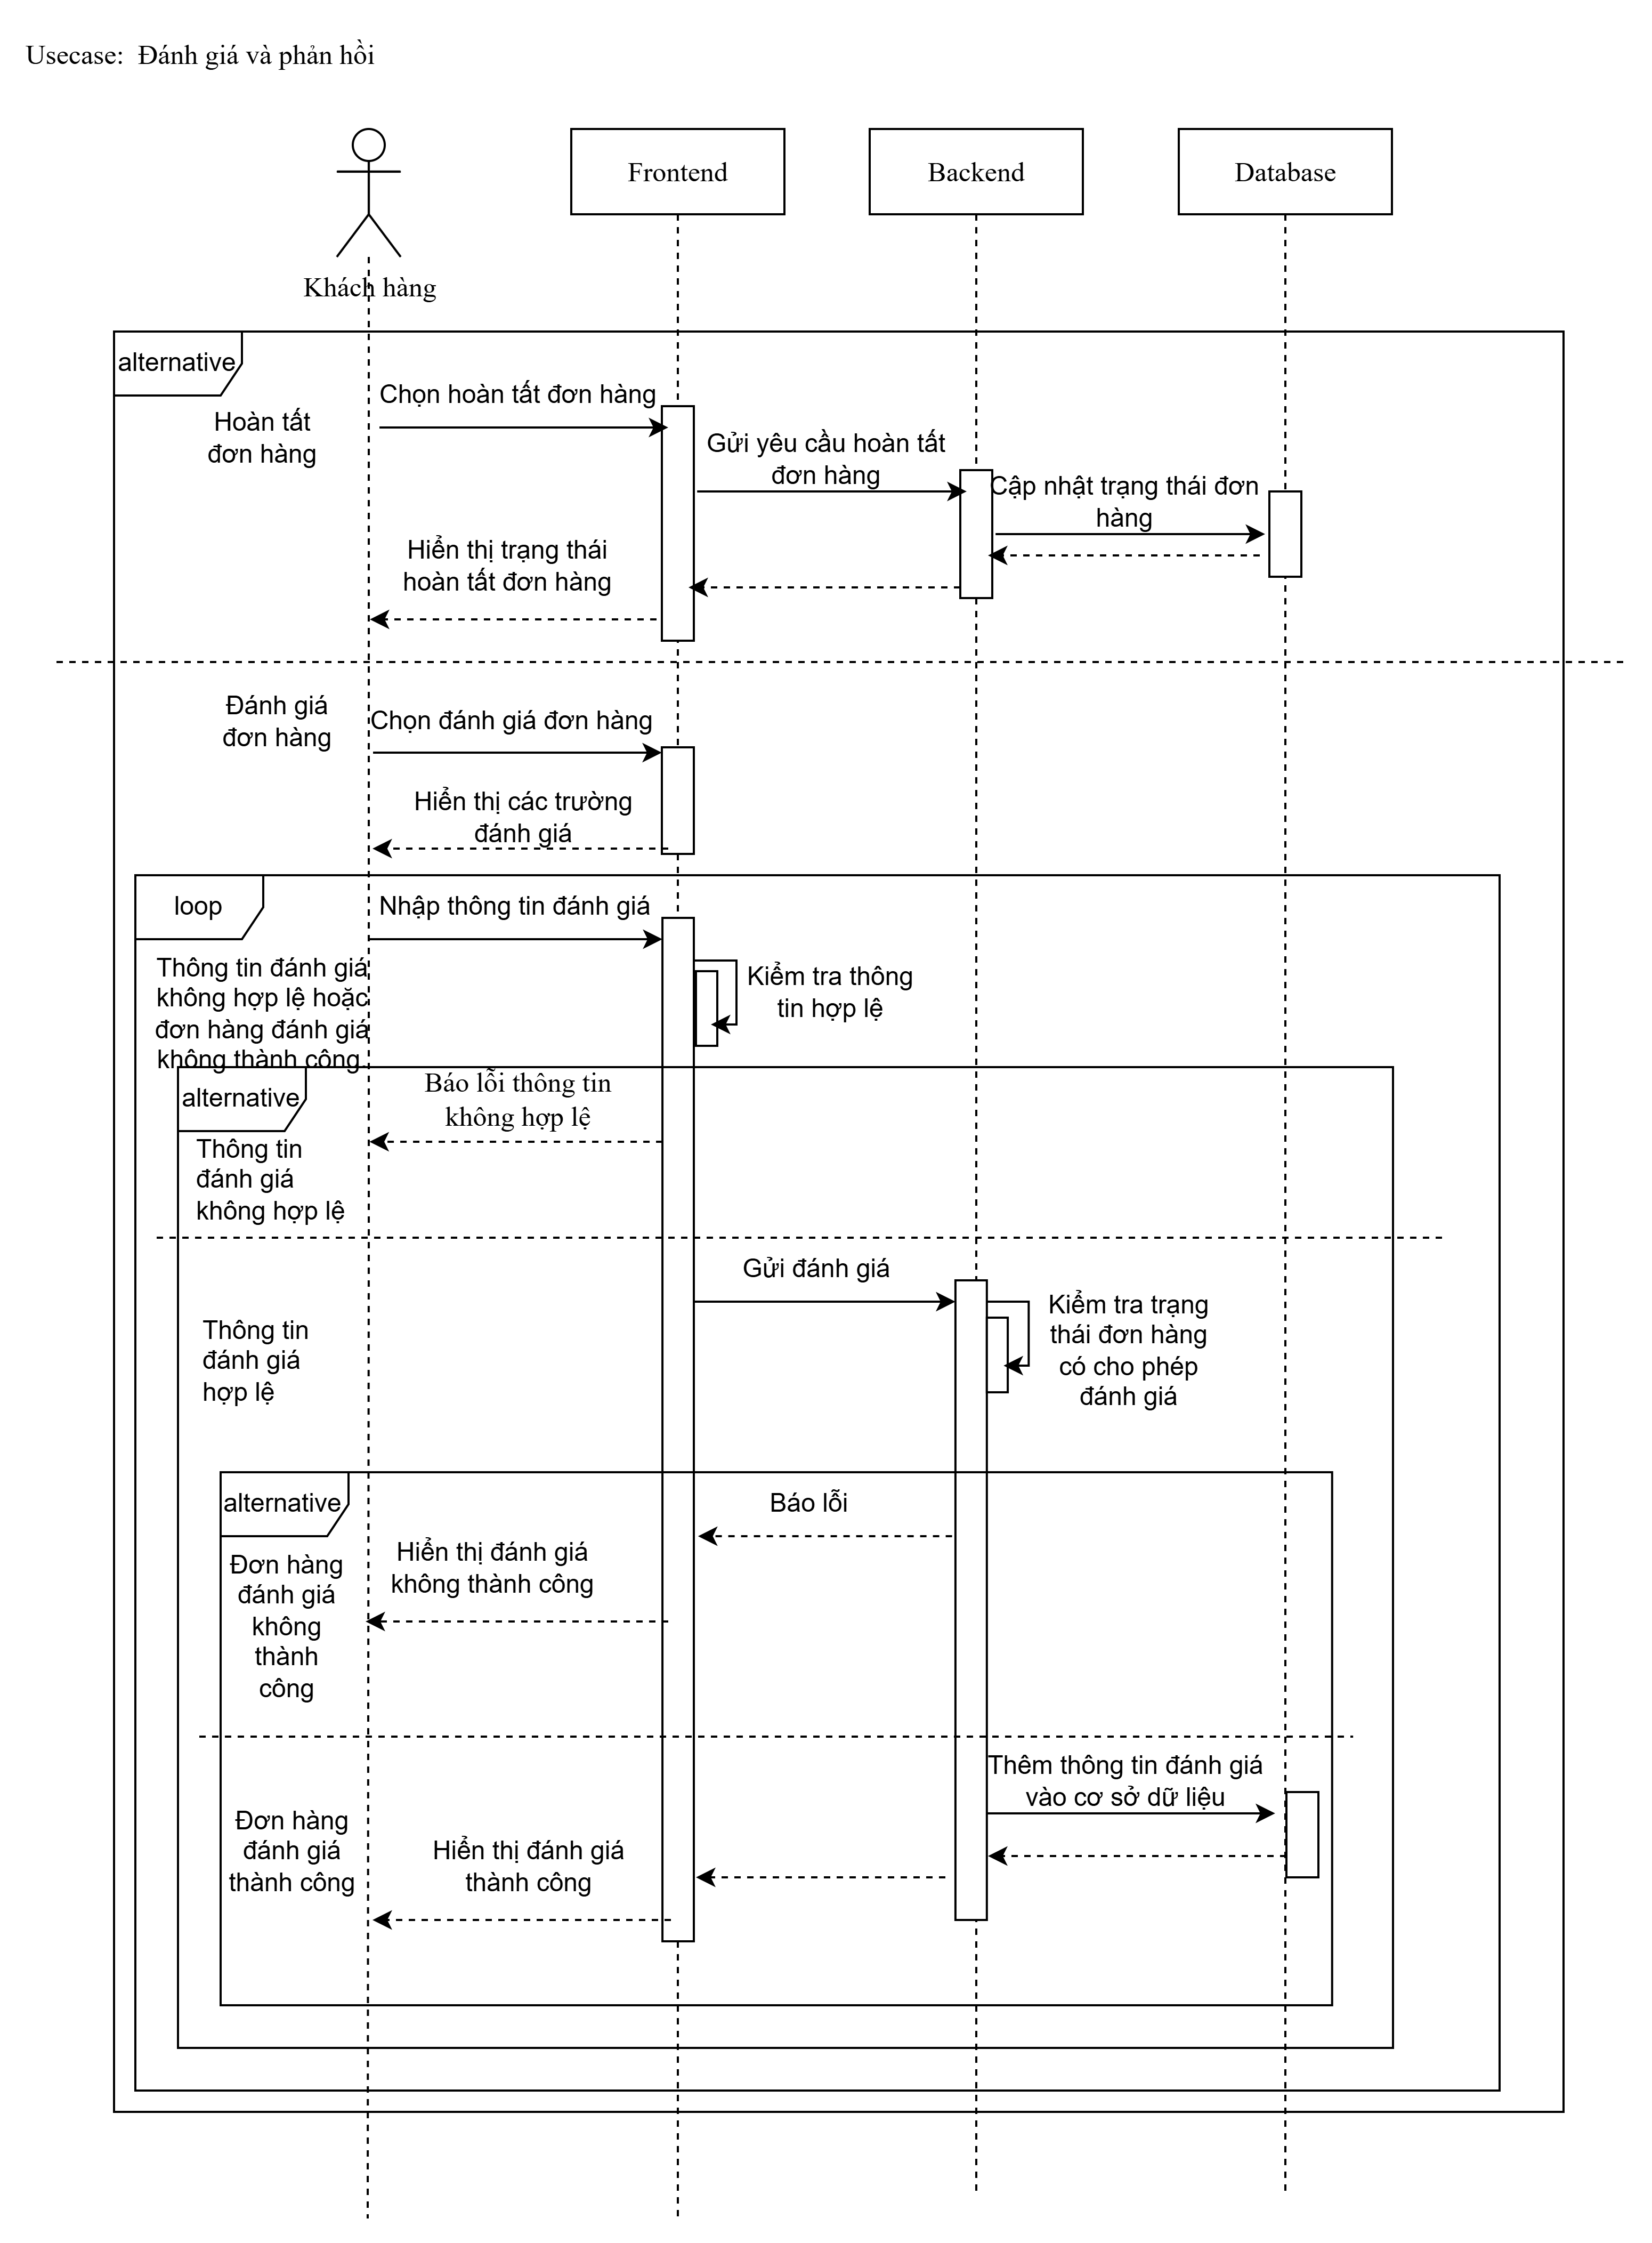
\includegraphics[width=0.9\linewidth]{images/chap3/sequence_diagram/customer_feedback.png}
   \vspace{0.5cm} \caption{Sơ đồ tuần tự Gửi phản hồi khách hàng}
    \label{fig:seq_feedback}
\end{figure}
Sau khi hoàn tất đơn hàng, người dùng gửi đánh giá. Hệ thống lưu trữ nội dung phản hồi và liên kết nó với sản phẩm hoặc đơn hàng tương ứng trong cơ sở dữ liệu.

% --- NHÓM 4: DỊCH VỤ HỖ TRỢ (SUPPORT SERVICES) ---

\begin{figure}[H]
    \centering
    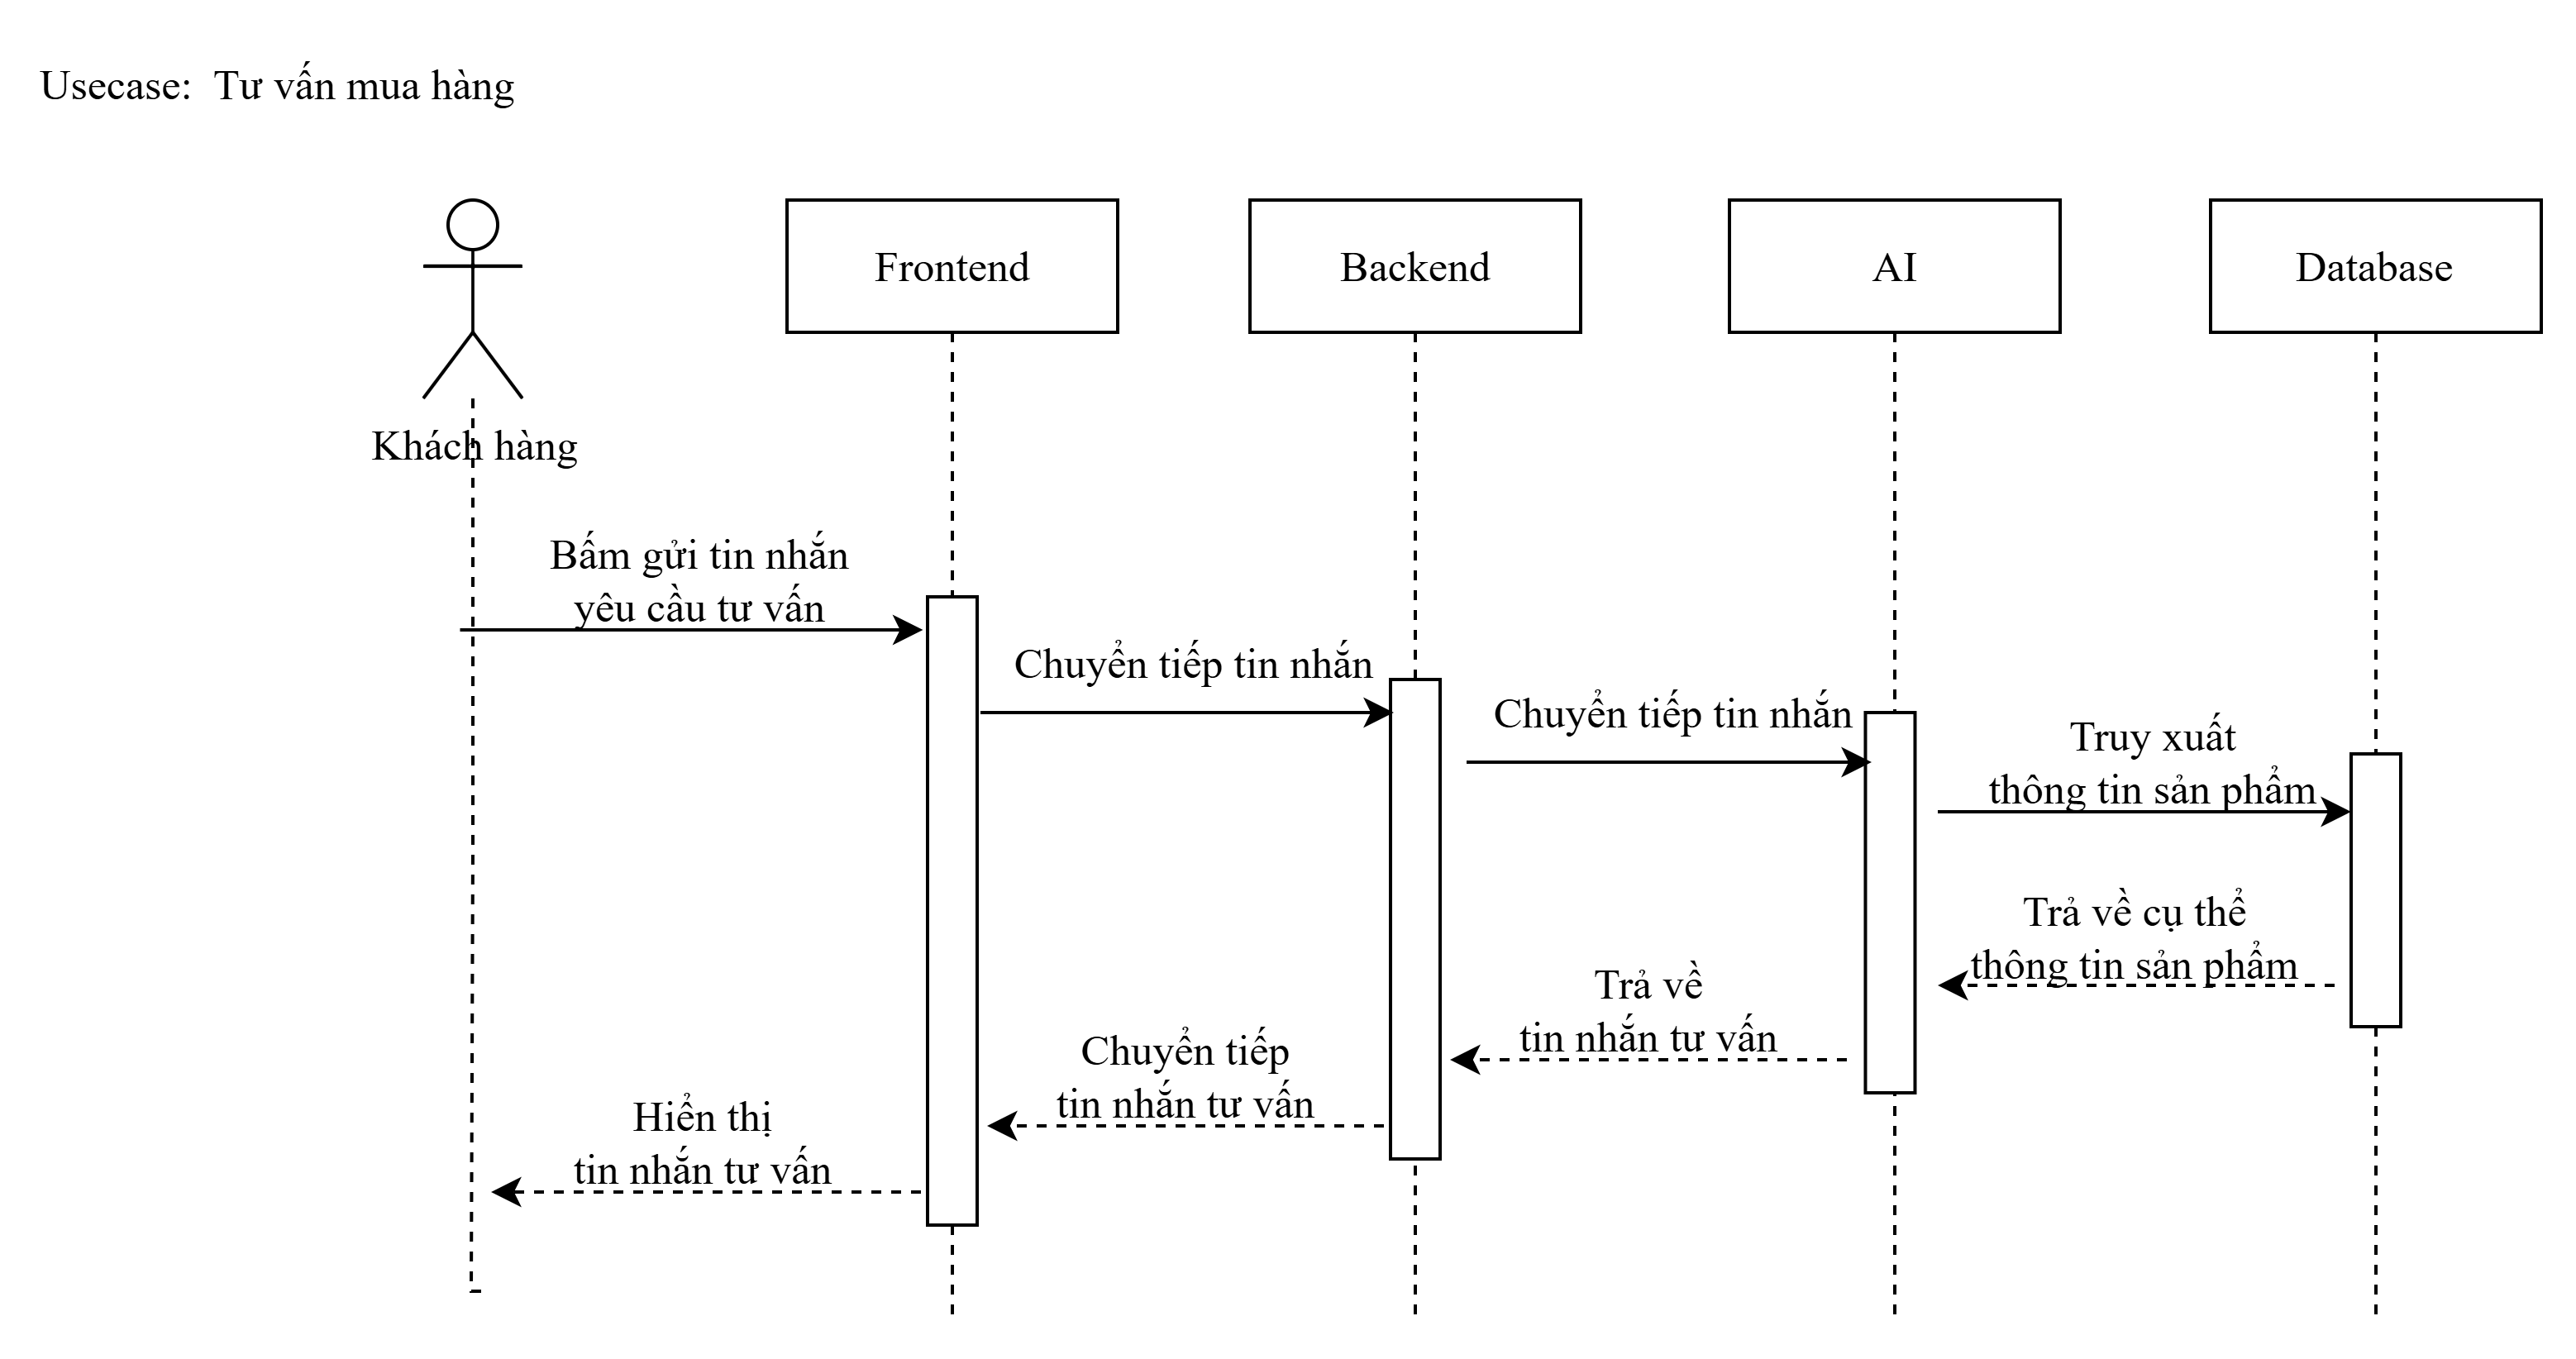
\includegraphics[width=0.9\linewidth]{images/chap3/sequence_diagram/shopping_consulting.png}
   \vspace{0.5cm} \caption{Sơ đồ tuần tự Tư vấn mua sắm}
    \label{fig:seq_consulting}
\end{figure}
Mô tả luồng tin nhắn giữa Khách hàng và Nhân viên hỗ trợ/Hệ thống Chatbot để giải đáp thắc mắc về sản phẩm trước khi mua.

\begin{figure}[H]
    \centering
    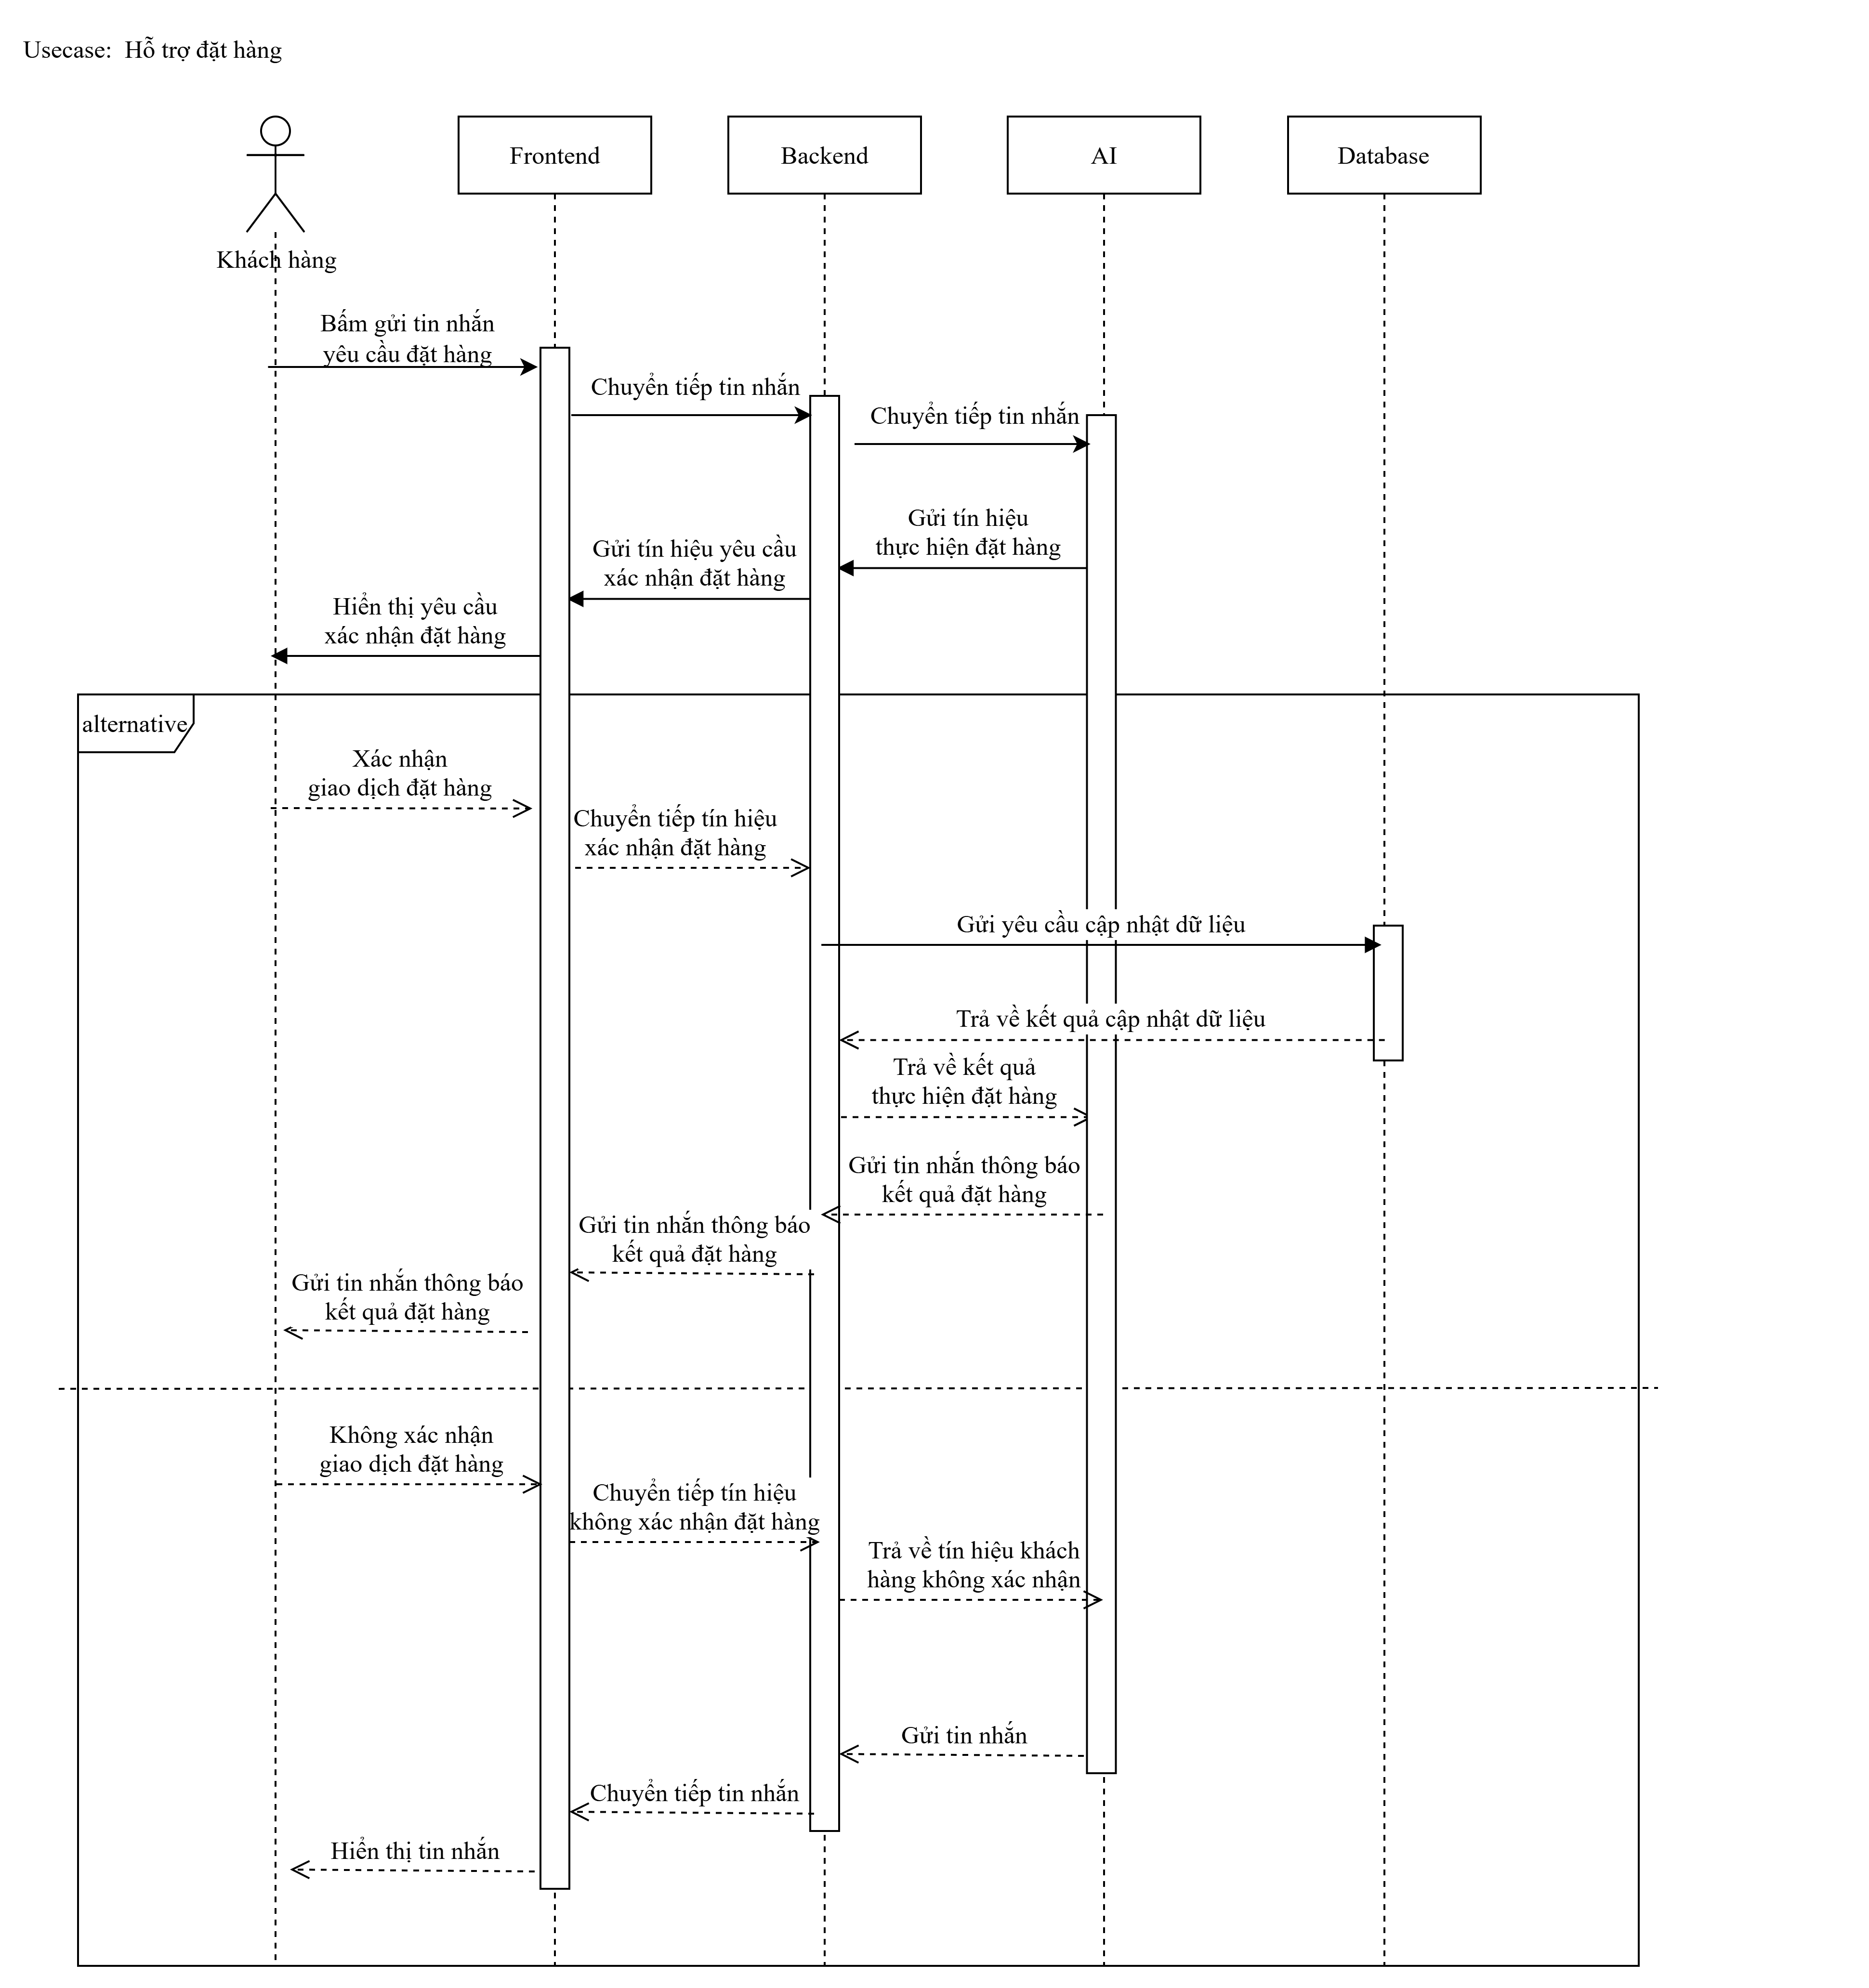
\includegraphics[width=0.9\linewidth]{images/chap3/sequence_diagram/place_order_support.png}
   \vspace{0.5cm} \caption{Sơ đồ tuần tự Hỗ trợ đặt hàng}
    \label{fig:seq_support_place}
\end{figure}
Nhân viên hỗ trợ tiếp nhận thông tin từ khách hàng, thay mặt khách hàng tương tác với hệ thống để thực hiện quy trình tạo đơn hàng (thường dùng trong trường hợp khách gặp lỗi kỹ thuật).

\begin{figure}[H]
    \centering
    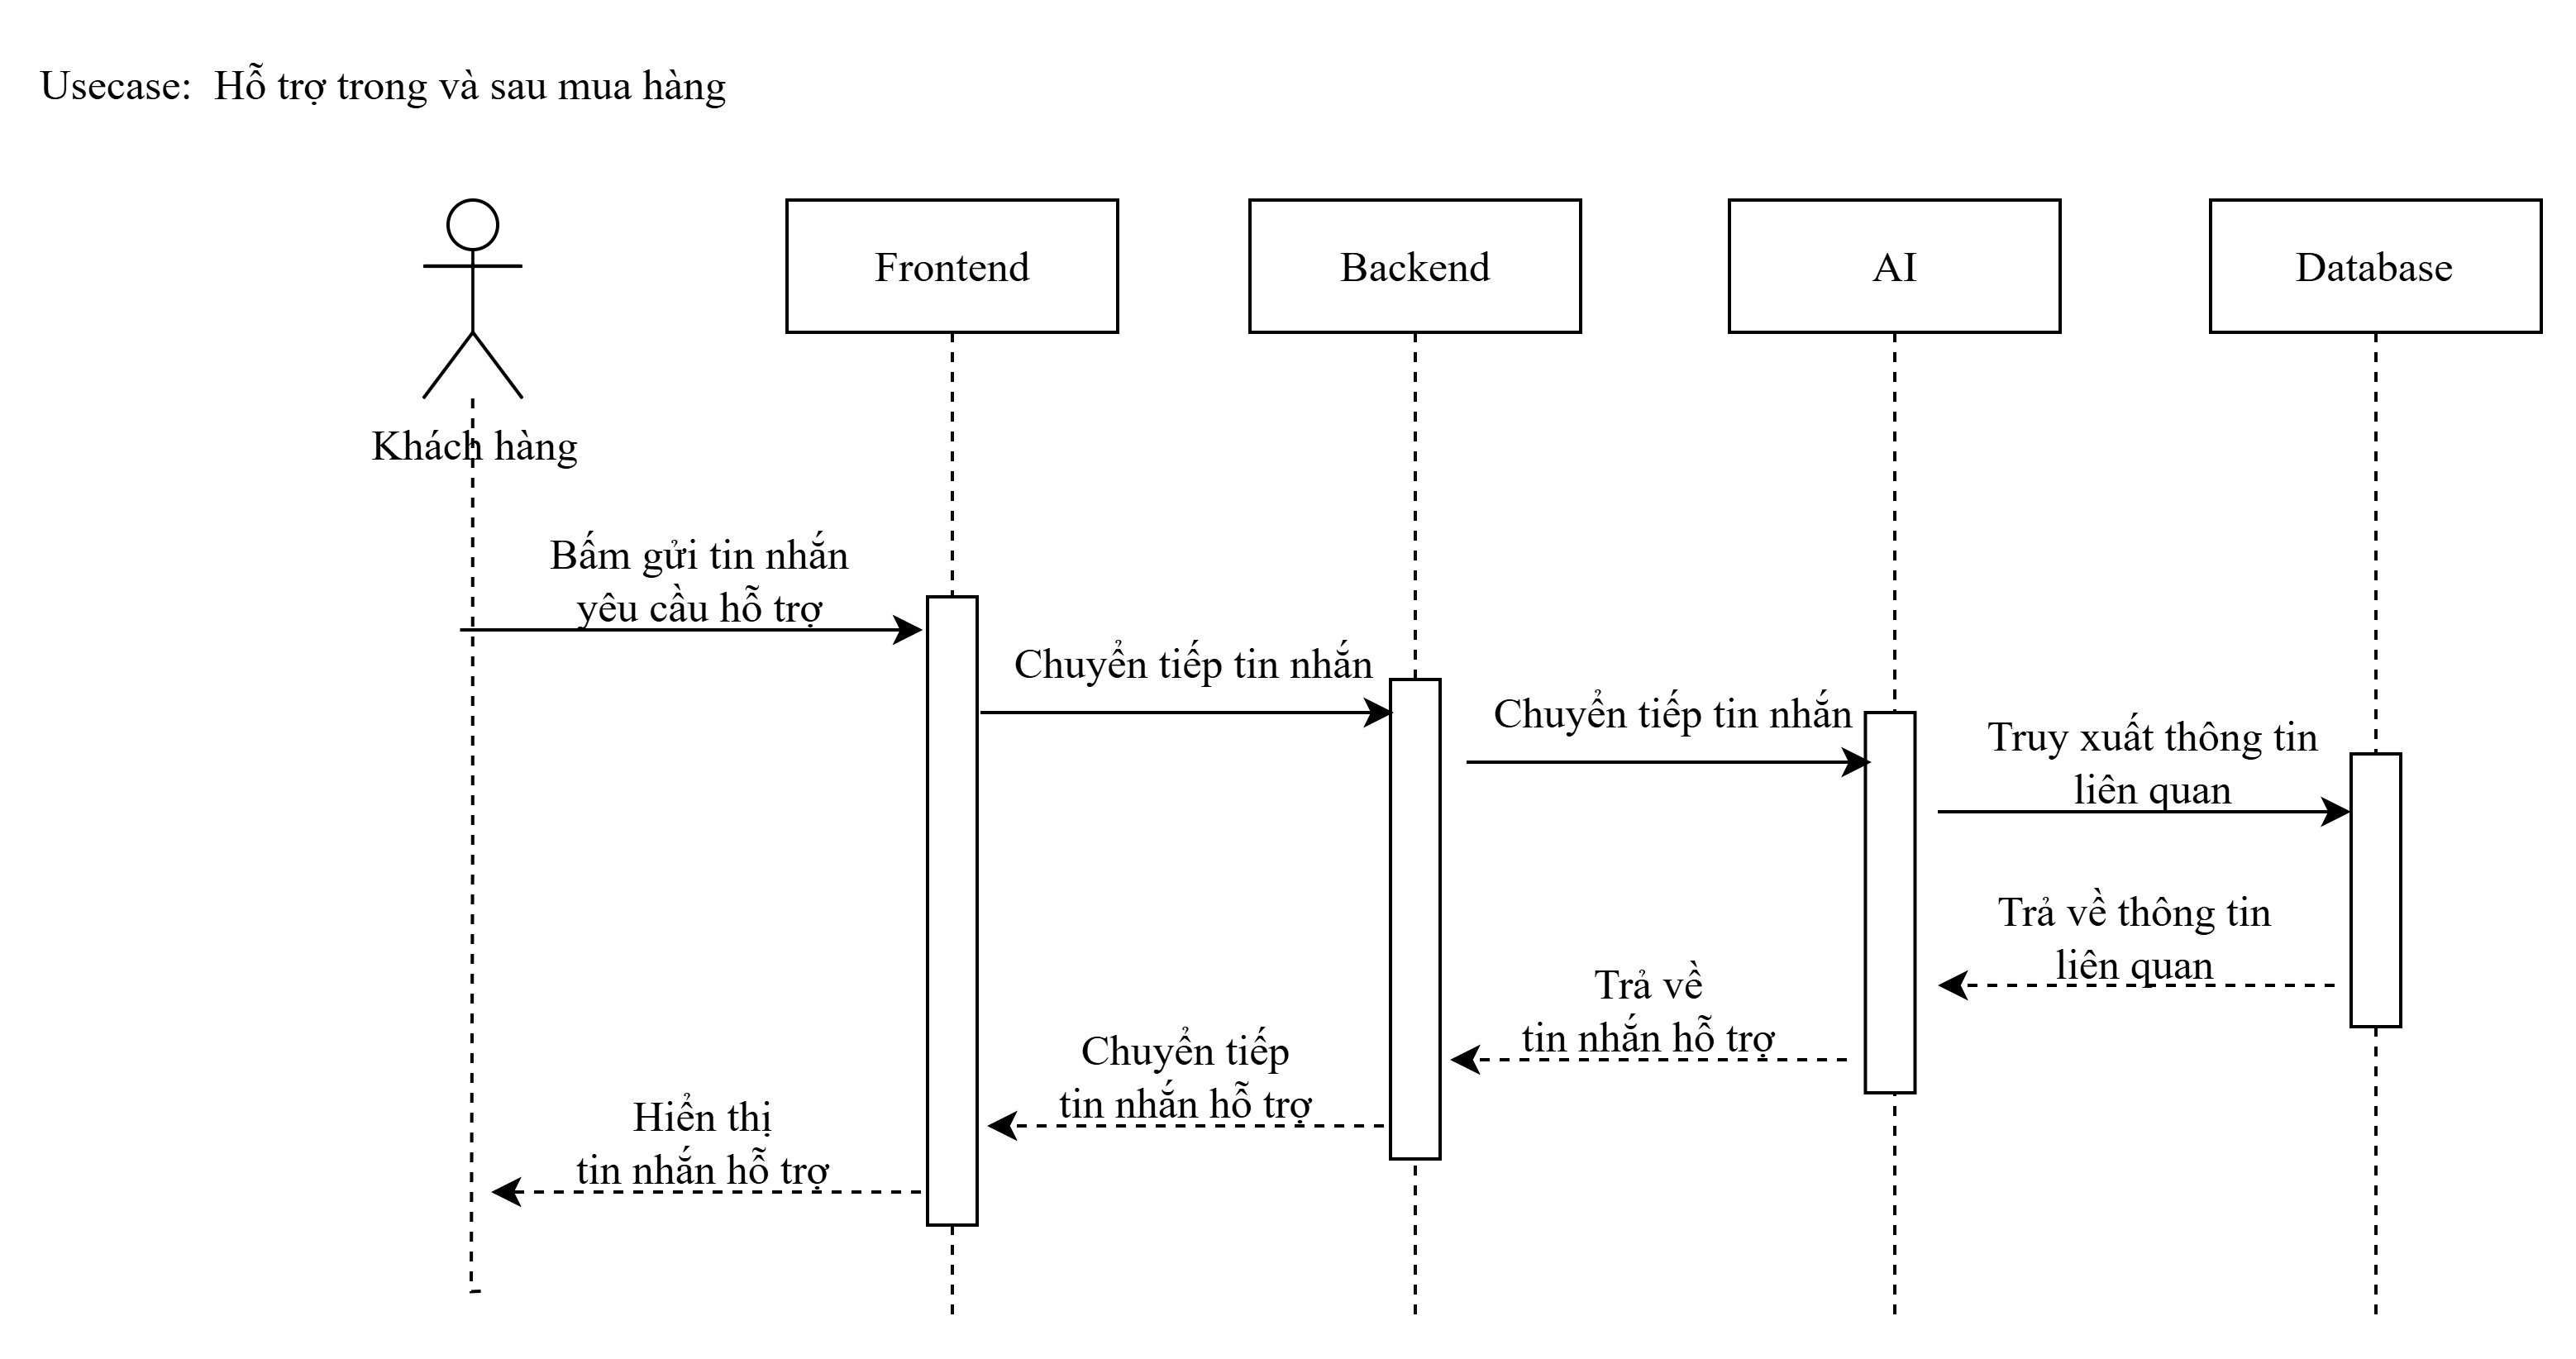
\includegraphics[width=0.9\linewidth]{images/chap3/sequence_diagram/shopping_support.png}
   \vspace{0.5cm} \caption{Sơ đồ tuần tự Hỗ trợ sau mua hàng}
    \label{fig:seq_shopping_support}
\end{figure}
Quy trình xử lý các khiếu nại hoặc yêu cầu bảo hành. Nhân viên kiểm tra thông tin đơn hàng trên hệ thống và ghi nhận kết quả xử lý hỗ trợ.

\begin{figure}[H]
    \centering
    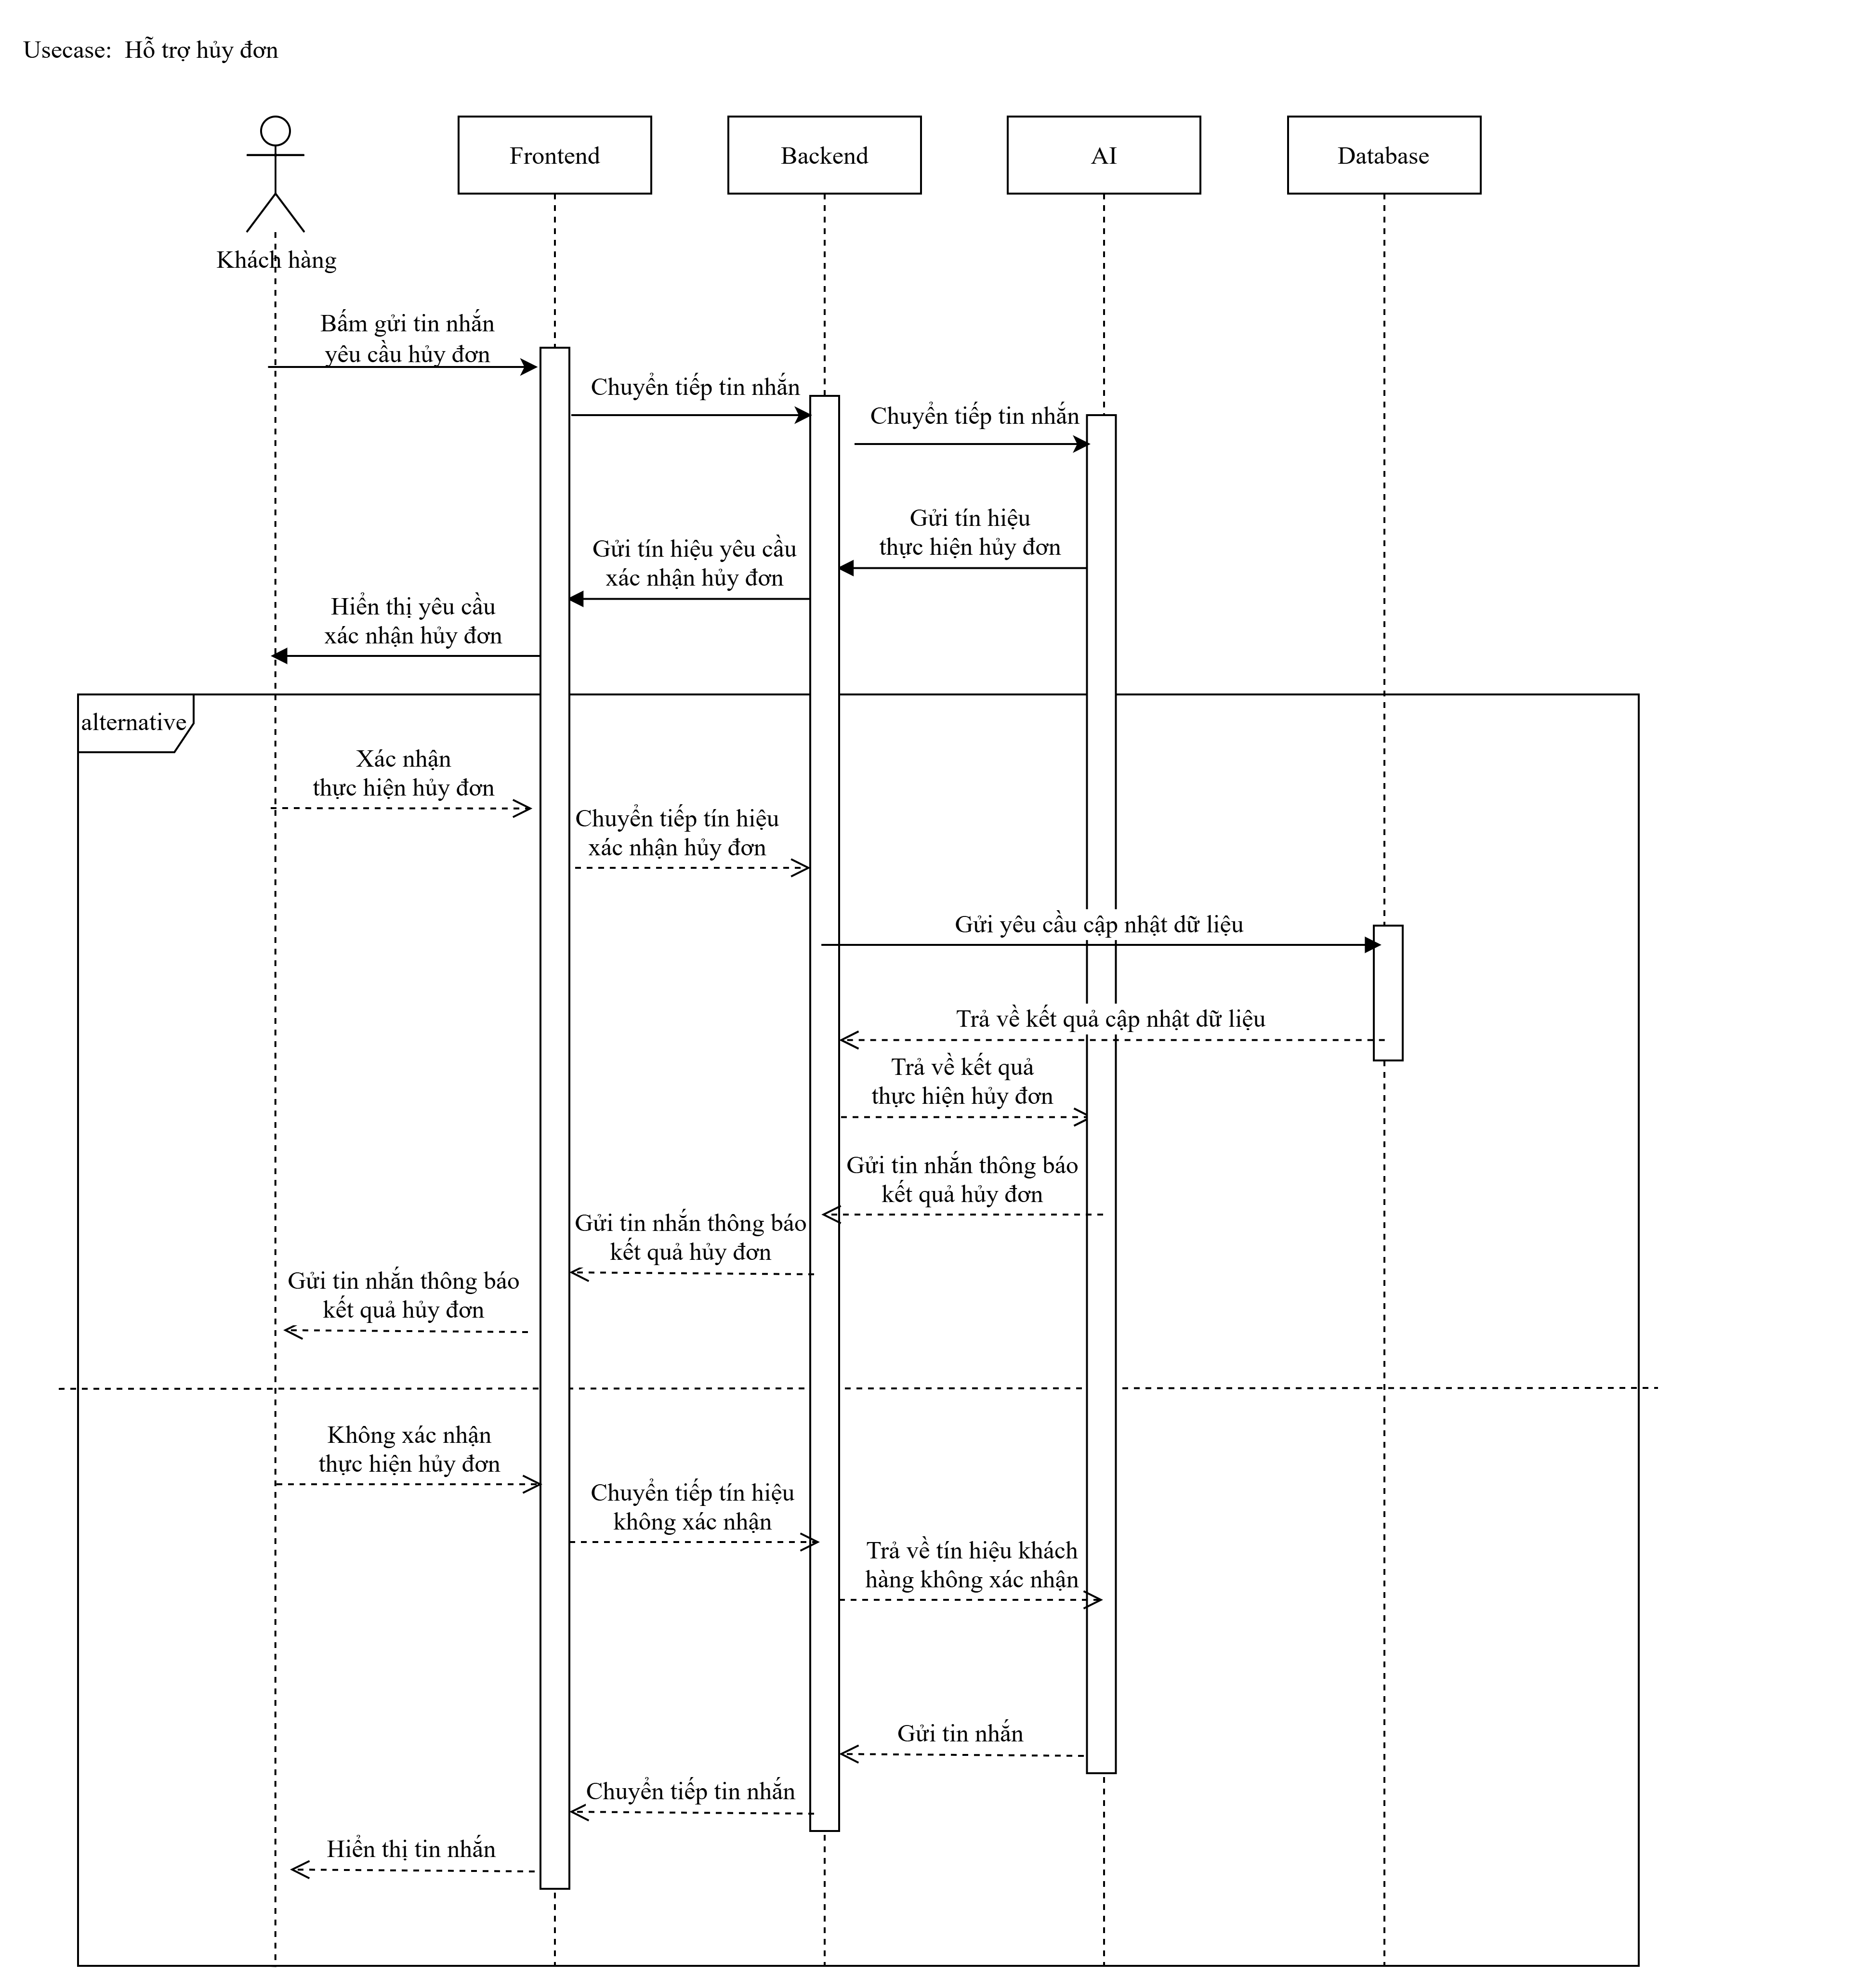
\includegraphics[width=0.9\linewidth]{images/chap3/sequence_diagram/cancel_order_support.png}
   \vspace{0.5cm} \caption{Sơ đồ tuần tự Hỗ trợ hủy đơn hàng}
    \label{fig:seq_support_cancel}
\end{figure}
Nhân viên hỗ trợ tiếp nhận yêu cầu hủy từ khách, thực hiện thao tác hủy trên hệ thống quản trị và kích hoạt quy trình hoàn tiền (nếu có).

% --- NHÓM 5: QUẢN TRỊ HỆ THỐNG (ADMINISTRATION) ---

\begin{figure}[H]
    \centering
    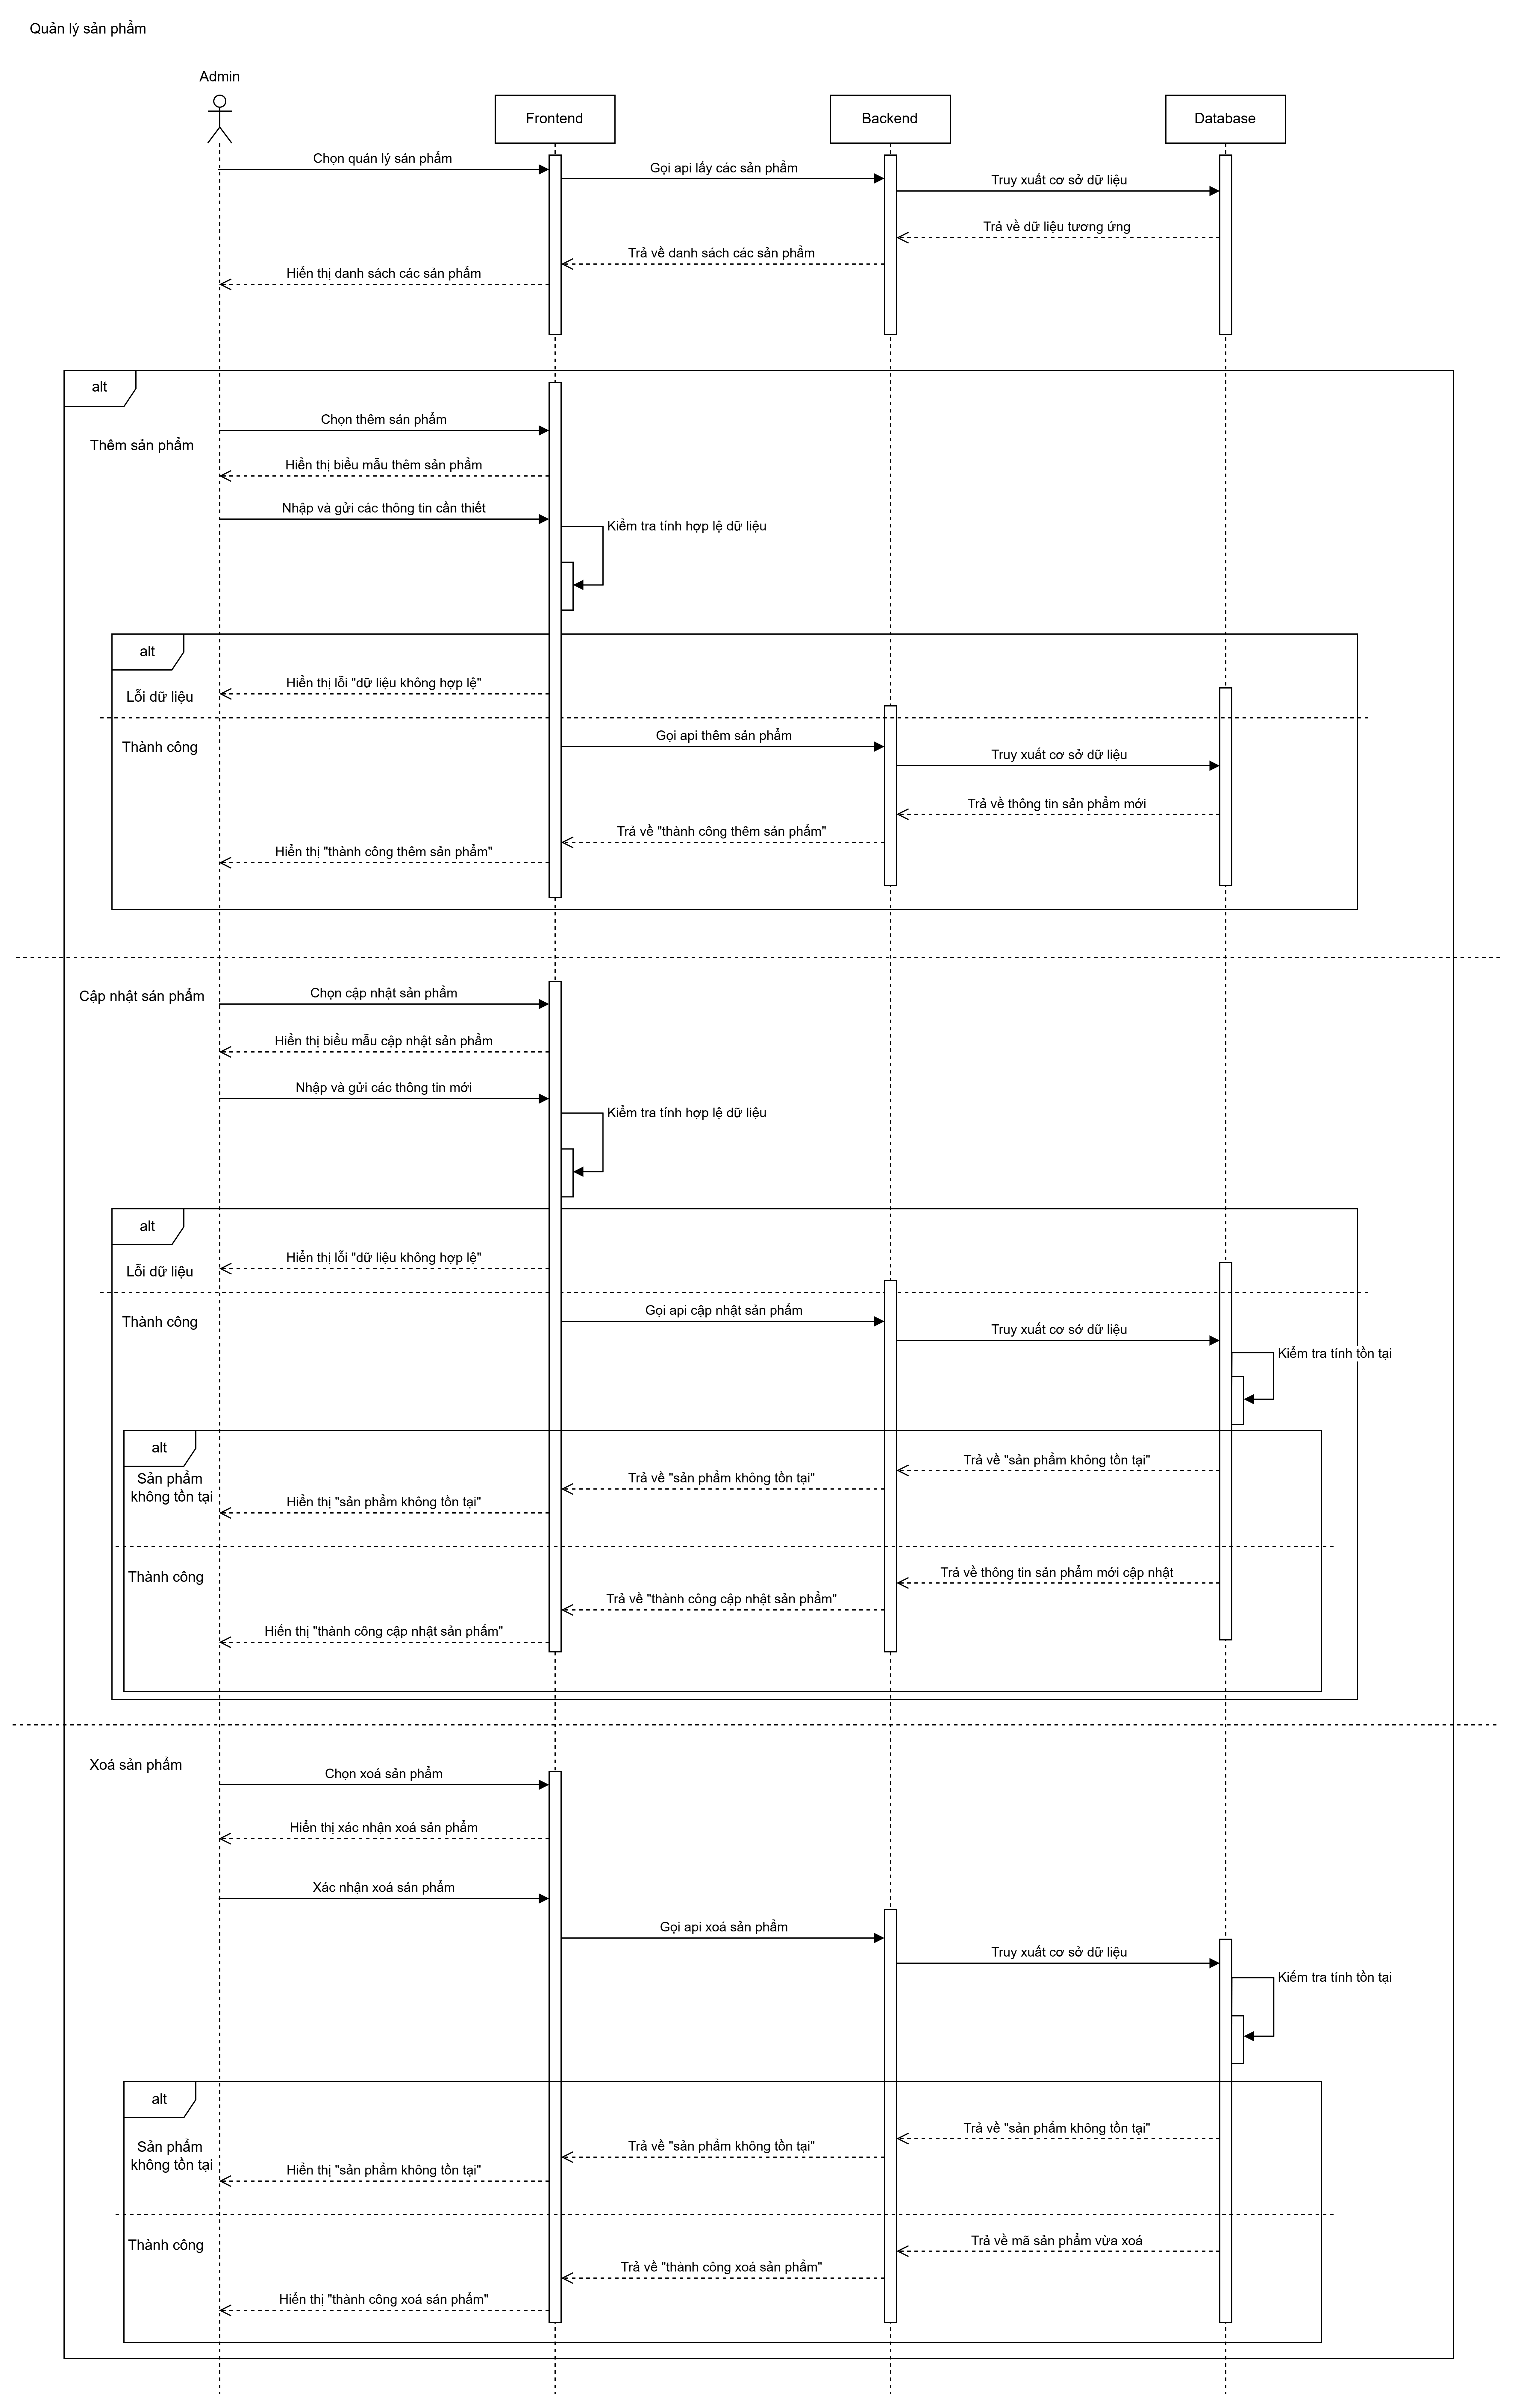
\includegraphics[width=1.0\linewidth]{images/chap3/sequence_diagram/manage_product.png}
   \vspace{0.5cm} \caption{Sơ đồ tuần tự Quản lý sản phẩm}
    \label{fig:seq_manage_product}
\end{figure}
Admin gửi yêu cầu Thêm/Sửa/Xóa. Hệ thống thực hiện Validate dữ liệu đầu vào, sau đó thực hiện lệnh SQL tương ứng xuống Database và trả về kết quả cập nhật danh sách sản phẩm.


\begin{figure}[H]
    \centering
    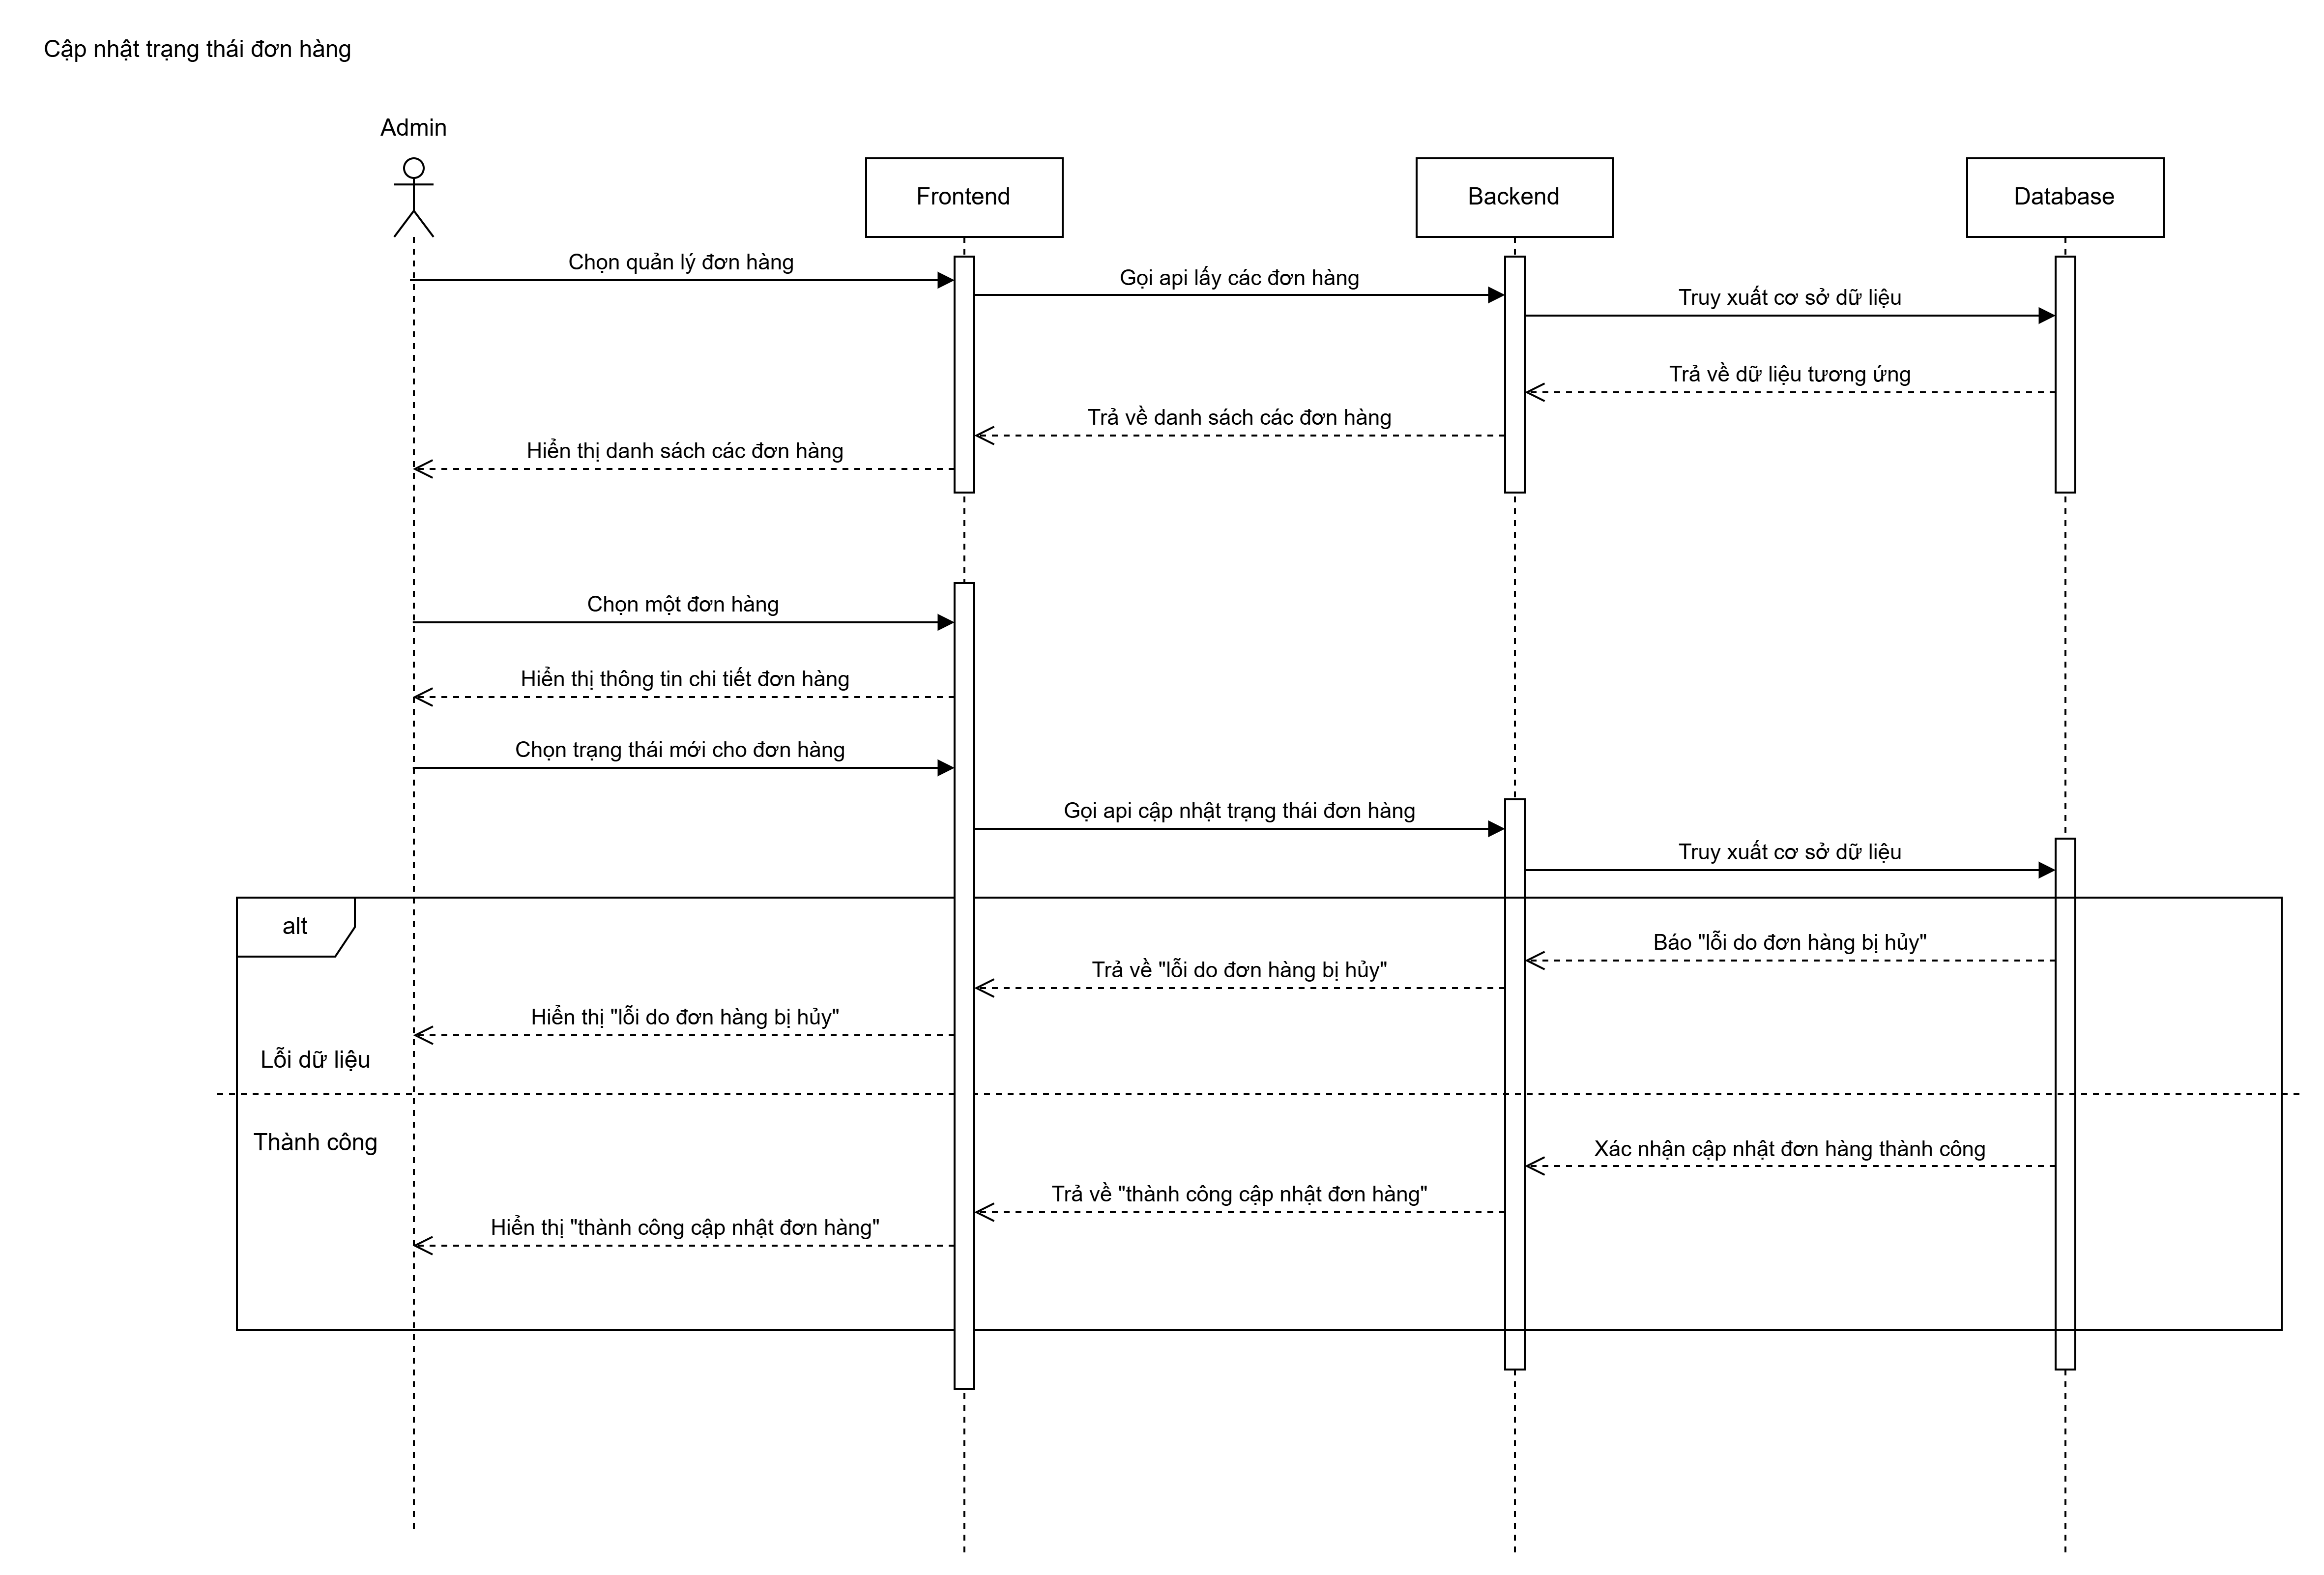
\includegraphics[width=0.9\linewidth]{images/chap3/sequence_diagram/change_order_status.png}
   \vspace{0.5cm} \caption{Sơ đồ tuần tự Cập nhật trạng thái đơn hàng}
    \label{fig:seq_change_status}
\end{figure}
Admin chọn đơn hàng và trạng thái mới (ví dụ: Xác nhận -> Đang giao). Hệ thống cập nhật bản ghi trong Database và có thể kích hoạt gửi email thông báo cho khách hàng.

\begin{figure}[H]
    \centering
    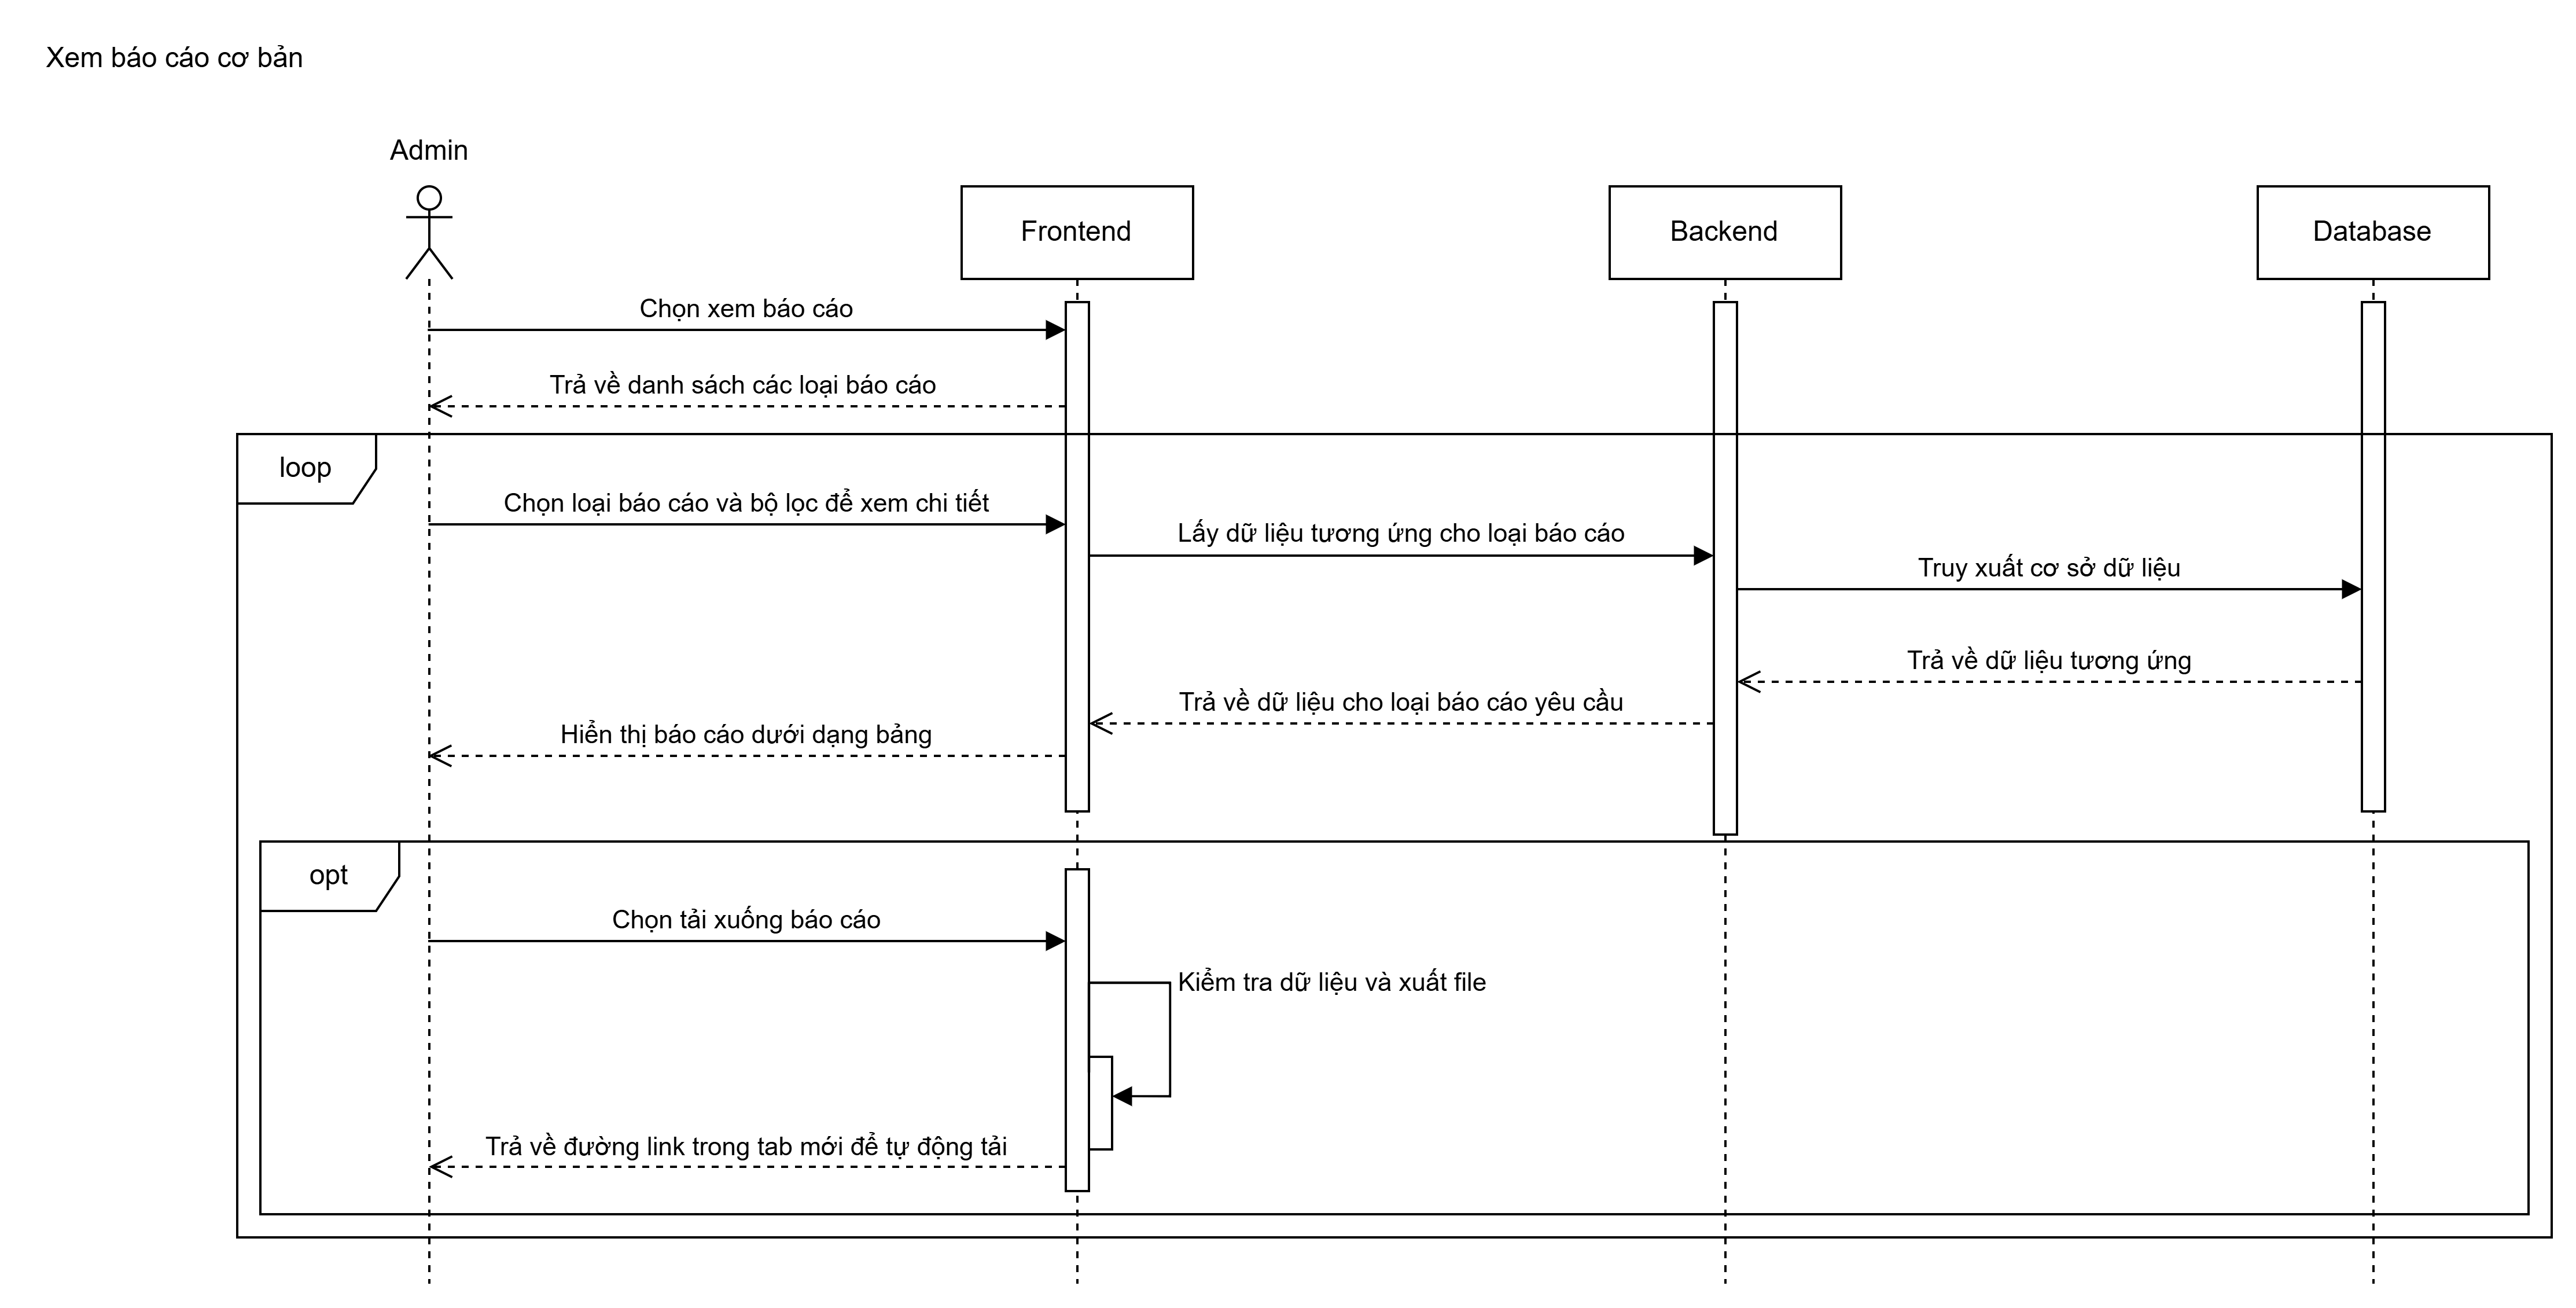
\includegraphics[width=0.9\linewidth]{images/chap3/sequence_diagram/view_basic_report.png}
   \vspace{0.5cm} \caption{Sơ đồ tuần tự Xem báo cáo thống kê}
    \label{fig:seq_report}
\end{figure}
Admin chọn loại báo cáo và khoảng thời gian. Hệ thống tổng hợp dữ liệu từ các bảng Order, Product, Payment,... tính toán các chỉ số và hiển thị biểu đồ hoặc bảng số liệu.
